\documentclass[twoside]{book}

% Packages required by doxygen
\usepackage{fixltx2e}
\usepackage{calc}
\usepackage{doxygen}
\usepackage[export]{adjustbox} % also loads graphicx
\usepackage{graphicx}
\usepackage[utf8]{inputenc}
\usepackage{makeidx}
\usepackage{multicol}
\usepackage{multirow}
\PassOptionsToPackage{warn}{textcomp}
\usepackage{textcomp}
\usepackage[nointegrals]{wasysym}
\usepackage[table]{xcolor}

% Font selection
\usepackage[T1]{fontenc}
\usepackage[scaled=.90]{helvet}
\usepackage{courier}
\usepackage{amssymb}
\usepackage{sectsty}
\renewcommand{\familydefault}{\sfdefault}
\allsectionsfont{%
  \fontseries{bc}\selectfont%
  \color{darkgray}%
}
\renewcommand{\DoxyLabelFont}{%
  \fontseries{bc}\selectfont%
  \color{darkgray}%
}
\newcommand{\+}{\discretionary{\mbox{\scriptsize$\hookleftarrow$}}{}{}}

% Page & text layout
\usepackage{geometry}
\geometry{%
  a4paper,%
  top=2.5cm,%
  bottom=2.5cm,%
  left=2.5cm,%
  right=2.5cm%
}
\tolerance=750
\hfuzz=15pt
\hbadness=750
\setlength{\emergencystretch}{15pt}
\setlength{\parindent}{0cm}
\setlength{\parskip}{3ex plus 2ex minus 2ex}
\makeatletter
\renewcommand{\paragraph}{%
  \@startsection{paragraph}{4}{0ex}{-1.0ex}{1.0ex}{%
    \normalfont\normalsize\bfseries\SS@parafont%
  }%
}
\renewcommand{\subparagraph}{%
  \@startsection{subparagraph}{5}{0ex}{-1.0ex}{1.0ex}{%
    \normalfont\normalsize\bfseries\SS@subparafont%
  }%
}
\makeatother

% Headers & footers
\usepackage{fancyhdr}
\pagestyle{fancyplain}
\fancyhead[LE]{\fancyplain{}{\bfseries\thepage}}
\fancyhead[CE]{\fancyplain{}{}}
\fancyhead[RE]{\fancyplain{}{\bfseries\leftmark}}
\fancyhead[LO]{\fancyplain{}{\bfseries\rightmark}}
\fancyhead[CO]{\fancyplain{}{}}
\fancyhead[RO]{\fancyplain{}{\bfseries\thepage}}
\fancyfoot[LE]{\fancyplain{}{}}
\fancyfoot[CE]{\fancyplain{}{}}
\fancyfoot[RE]{\fancyplain{}{\bfseries\scriptsize Generated by Doxygen }}
\fancyfoot[LO]{\fancyplain{}{\bfseries\scriptsize Generated by Doxygen }}
\fancyfoot[CO]{\fancyplain{}{}}
\fancyfoot[RO]{\fancyplain{}{}}
\renewcommand{\footrulewidth}{0.4pt}
\renewcommand{\chaptermark}[1]{%
  \markboth{#1}{}%
}
\renewcommand{\sectionmark}[1]{%
  \markright{\thesection\ #1}%
}

% Indices & bibliography
\usepackage{natbib}
\usepackage[titles]{tocloft}
\setcounter{tocdepth}{3}
\setcounter{secnumdepth}{5}
\makeindex

% Hyperlinks (required, but should be loaded last)
\usepackage{ifpdf}
\ifpdf
  \usepackage[pdftex,pagebackref=true]{hyperref}
\else
  \usepackage[ps2pdf,pagebackref=true]{hyperref}
\fi
\hypersetup{%
  colorlinks=true,%
  linkcolor=blue,%
  citecolor=blue,%
  unicode%
}

% Custom commands
\newcommand{\clearemptydoublepage}{%
  \newpage{\pagestyle{empty}\cleardoublepage}%
}

\usepackage{caption}
\captionsetup{labelsep=space,justification=centering,font={bf},singlelinecheck=off,skip=4pt,position=top}

%===== C O N T E N T S =====

\begin{document}

% Titlepage & ToC
\hypersetup{pageanchor=false,
             bookmarksnumbered=true,
             pdfencoding=unicode
            }
\pagenumbering{alph}
\begin{titlepage}
\vspace*{7cm}
\begin{center}%
{\Large vsrs \\[1ex]\large 4.\+2 }\\
\vspace*{1cm}
{\large Generated by Doxygen 1.8.13}\\
\end{center}
\end{titlepage}
\clearemptydoublepage
\pagenumbering{roman}
\tableofcontents
\clearemptydoublepage
\pagenumbering{arabic}
\hypersetup{pageanchor=true}

%--- Begin generated contents ---
\chapter{V\+S\+RS and D\+E\+RS}
\label{md__i_1__v_s_r_s4_vsrs__readme}
\Hypertarget{md__i_1__v_s_r_s4_vsrs__readme}
\subsection*{How to clone from the official repository}

This repository is a copy of the original one arount january 2016

\subsubsection*{Identification}

user\+: mpeg-\/ftv

pass\+: ftvftv

\subsubsection*{Git cloning}


\begin{DoxyCode}
git svn clone --username=mpeg-ftv https://svn.multimedia.edu.pl/vsrs
git svn clone --username=mpeg-ftv https://svn.multimedia.edu.pl/ders
git svn clone --username=mpeg-ftv https://svn.multimedia.edu.pl/mpeg-ftv
\end{DoxyCode}


\subsubsection*{publication from\+:}

\href{publications-2013-MPEG_M31520.pdf}{\tt http\+://www.\+multimedia.\+edu.\+pl/publications/\+M\+P\+E\+G\+\_\+\+M31520-\/\+Enhanced-\/\+View-\/\+Synthesis-\/\+Reference-\/\+Software-\/\+V\+S\+R\+S-\/for-\/\+Free-\/viewpoint-\/television.\+pdf} 
\chapter{Hierarchical Index}
\section{Class Hierarchy}
This inheritance list is sorted roughly, but not completely, alphabetically\+:\begin{DoxyCompactList}
\item \contentsline{section}{C\+Boundary\+Noise\+Removal}{\pageref{class_c_boundary_noise_removal}}{}
\item \contentsline{section}{C\+Camera\+Parameters}{\pageref{class_c_camera_parameters}}{}
\item \contentsline{section}{C\+I\+Yuv$<$ Pixel\+Type $>$}{\pageref{class_c_i_yuv}}{}
\item \contentsline{section}{C\+I\+Yuv$<$ Depth\+Type $>$}{\pageref{class_c_i_yuv}}{}
\item \contentsline{section}{C\+I\+Yuv$<$ Image\+Type $>$}{\pageref{class_c_i_yuv}}{}
\item \contentsline{section}{Config\+Line\+Base}{\pageref{class_config_line_base}}{}
\begin{DoxyCompactList}
\item \contentsline{section}{Config\+Line\+Char}{\pageref{class_config_line_char}}{}
\item \contentsline{section}{Config\+Line\+Dbl}{\pageref{class_config_line_dbl}}{}
\item \contentsline{section}{Config\+Line\+Int}{\pageref{class_config_line_int}}{}
\item \contentsline{section}{Config\+Line\+Str}{\pageref{class_config_line_str}}{}
\item \contentsline{section}{Config\+Line\+U\+Int}{\pageref{class_config_line_u_int}}{}
\end{DoxyCompactList}
\item \contentsline{section}{C\+Picture\+Resample$<$ Pixel\+Type $>$}{\pageref{class_c_picture_resample}}{}
\item \contentsline{section}{C\+View\+Interpolation}{\pageref{class_c_view_interpolation}}{}
\item \contentsline{section}{C\+View\+Interpolation1D}{\pageref{class_c_view_interpolation1_d}}{}
\item \contentsline{section}{C\+View\+Interpolation\+General}{\pageref{class_c_view_interpolation_general}}{}
\item \contentsline{section}{Parameter\+Base}{\pageref{class_parameter_base}}{}
\begin{DoxyCompactList}
\item \contentsline{section}{C\+Parameter\+View\+Interpolation}{\pageref{class_c_parameter_view_interpolation}}{}
\end{DoxyCompactList}
\end{DoxyCompactList}

\chapter{Class Index}
\section{Class List}
Here are the classes, structs, unions and interfaces with brief descriptions\+:\begin{DoxyCompactList}
\item\contentsline{section}{\hyperlink{class_c_boundary_noise_removal}{C\+Boundary\+Noise\+Removal} }{\pageref{class_c_boundary_noise_removal}}{}
\item\contentsline{section}{\hyperlink{class_c_camera_parameters}{C\+Camera\+Parameters} }{\pageref{class_c_camera_parameters}}{}
\item\contentsline{section}{\hyperlink{class_c_i_yuv}{C\+I\+Yuv$<$ Pixel\+Type $>$} }{\pageref{class_c_i_yuv}}{}
\item\contentsline{section}{\hyperlink{class_config_line_base}{Config\+Line\+Base} }{\pageref{class_config_line_base}}{}
\item\contentsline{section}{\hyperlink{class_config_line_char}{Config\+Line\+Char} \\*\hyperlink{class_config_line_char}{Config\+Line\+Char} -\/ char }{\pageref{class_config_line_char}}{}
\item\contentsline{section}{\hyperlink{class_config_line_dbl}{Config\+Line\+Dbl} \\*\hyperlink{class_config_line_dbl}{Config\+Line\+Dbl} -\/ double }{\pageref{class_config_line_dbl}}{}
\item\contentsline{section}{\hyperlink{class_config_line_int}{Config\+Line\+Int} \\*\hyperlink{class_config_line_int}{Config\+Line\+Int} -\/ int }{\pageref{class_config_line_int}}{}
\item\contentsline{section}{\hyperlink{class_config_line_str}{Config\+Line\+Str} \\*\hyperlink{class_config_line_str}{Config\+Line\+Str} -\/ string }{\pageref{class_config_line_str}}{}
\item\contentsline{section}{\hyperlink{class_config_line_u_int}{Config\+Line\+U\+Int} \\*\hyperlink{class_config_line_u_int}{Config\+Line\+U\+Int} -\/ uint }{\pageref{class_config_line_u_int}}{}
\item\contentsline{section}{\hyperlink{class_c_parameter_view_interpolation}{C\+Parameter\+View\+Interpolation} }{\pageref{class_c_parameter_view_interpolation}}{}
\item\contentsline{section}{\hyperlink{class_c_picture_resample}{C\+Picture\+Resample$<$ Pixel\+Type $>$} }{\pageref{class_c_picture_resample}}{}
\item\contentsline{section}{\hyperlink{class_c_view_interpolation}{C\+View\+Interpolation} }{\pageref{class_c_view_interpolation}}{}
\item\contentsline{section}{\hyperlink{class_c_view_interpolation1_d}{C\+View\+Interpolation1D} }{\pageref{class_c_view_interpolation1_d}}{}
\item\contentsline{section}{\hyperlink{class_c_view_interpolation_general}{C\+View\+Interpolation\+General} }{\pageref{class_c_view_interpolation_general}}{}
\item\contentsline{section}{\hyperlink{class_parameter_base}{Parameter\+Base} \\*\hyperlink{class_parameter_base}{Parameter\+Base} }{\pageref{class_parameter_base}}{}
\end{DoxyCompactList}

\chapter{Class Documentation}
\hypertarget{class_c_boundary_noise_removal}{}\section{C\+Boundary\+Noise\+Removal Class Reference}
\label{class_c_boundary_noise_removal}\index{C\+Boundary\+Noise\+Removal@{C\+Boundary\+Noise\+Removal}}
\subsection*{Public Member Functions}
\begin{DoxyCompactItemize}
\item 
\mbox{\Hypertarget{class_c_boundary_noise_removal_af789fb697fbb2919763b302dd7a1f59b}\label{class_c_boundary_noise_removal_af789fb697fbb2919763b302dd7a1f59b}} 
\hyperlink{class_c_boundary_noise_removal_af789fb697fbb2919763b302dd7a1f59b}{C\+Boundary\+Noise\+Removal} ()
\begin{DoxyCompactList}\small\item\em \begin{quote}
The real depth value of the farthest pixel. 0\+: Left view. 1\+: Right view \end{quote}
\end{DoxyCompactList}\item 
\mbox{\Hypertarget{class_c_boundary_noise_removal_a441713ad025973e9592dcd4b1825b1e3}\label{class_c_boundary_noise_removal_a441713ad025973e9592dcd4b1825b1e3}} 
bool {\bfseries Do\+Boundary\+Noise\+Removal} (\hyperlink{class_c_i_yuv}{C\+I\+Yuv}$<$ Image\+Type $>$ $\ast$p\+Ref\+Left, \hyperlink{class_c_i_yuv}{C\+I\+Yuv}$<$ Image\+Type $>$ $\ast$p\+Ref\+Right, \hyperlink{class_c_i_yuv}{C\+I\+Yuv}$<$ Depth\+Type $>$ $\ast$p\+Ref\+Depth\+Left, \hyperlink{class_c_i_yuv}{C\+I\+Yuv}$<$ Depth\+Type $>$ $\ast$p\+Ref\+Depth\+Right, \hyperlink{class_c_i_yuv}{C\+I\+Yuv}$<$ Hole\+Type $>$ $\ast$p\+Ref\+Hole\+Left, \hyperlink{class_c_i_yuv}{C\+I\+Yuv}$<$ Hole\+Type $>$ $\ast$p\+Ref\+Hole\+Right, \hyperlink{class_c_i_yuv}{C\+I\+Yuv}$<$ Image\+Type $>$ $\ast$p\+Syn\+Yuv\+Buffer, bool Synhtesis\+Mode)
\item 
\mbox{\Hypertarget{class_c_boundary_noise_removal_a1c1e4f5b6dd8ada3c20dbcaea0d55be7}\label{class_c_boundary_noise_removal_a1c1e4f5b6dd8ada3c20dbcaea0d55be7}} 
void {\bfseries x\+Init} ()
\item 
\mbox{\Hypertarget{class_c_boundary_noise_removal_a7a222f7088dc78c75bd89b89c5843edf}\label{class_c_boundary_noise_removal_a7a222f7088dc78c75bd89b89c5843edf}} 
void {\bfseries Set\+Width} (int i\+Width)
\item 
\mbox{\Hypertarget{class_c_boundary_noise_removal_ab07290b0fb9a1e5c8514ee0abe81e666}\label{class_c_boundary_noise_removal_ab07290b0fb9a1e5c8514ee0abe81e666}} 
void {\bfseries Set\+Height} (int i\+Hieght)
\item 
\mbox{\Hypertarget{class_c_boundary_noise_removal_af76af546229a18848870a63c05018b6e}\label{class_c_boundary_noise_removal_af76af546229a18848870a63c05018b6e}} 
void {\bfseries Set\+View\+Blending} (int b\+View\+Blending)
\item 
\mbox{\Hypertarget{class_c_boundary_noise_removal_a708dd37397392b52b9bf702318a670c0}\label{class_c_boundary_noise_removal_a708dd37397392b52b9bf702318a670c0}} 
void {\bfseries Set\+Color\+Space} (int b\+Color\+Space)
\item 
\mbox{\Hypertarget{class_c_boundary_noise_removal_ad062849b69c78cad7ddcb54994a63cc3}\label{class_c_boundary_noise_removal_ad062849b69c78cad7ddcb54994a63cc3}} 
void {\bfseries Set\+Precision} (int i\+Precision)
\item 
\mbox{\Hypertarget{class_c_boundary_noise_removal_a3b49c34d794bbc860e08b64520468b75}\label{class_c_boundary_noise_removal_a3b49c34d794bbc860e08b64520468b75}} 
void {\bfseries Set\+Left\+H\+\_\+\+V2R} (Cv\+Mat $\ast$s\+H\+\_\+\+V2R)
\item 
\mbox{\Hypertarget{class_c_boundary_noise_removal_ad7fc22b2351f439cb4d89f76ca13f92f}\label{class_c_boundary_noise_removal_ad7fc22b2351f439cb4d89f76ca13f92f}} 
void {\bfseries Set\+Right\+H\+\_\+\+V2R} (Cv\+Mat $\ast$s\+H\+\_\+\+V2R)
\item 
\mbox{\Hypertarget{class_c_boundary_noise_removal_aa1f94e9c908aac080ec5a45842596470}\label{class_c_boundary_noise_removal_aa1f94e9c908aac080ec5a45842596470}} 
void {\bfseries Set\+Focal\+Length} (double s\+Focal\+Length)
\item 
\mbox{\Hypertarget{class_c_boundary_noise_removal_a94183ffe9e6f8dff19e6321b959e313c}\label{class_c_boundary_noise_removal_a94183ffe9e6f8dff19e6321b959e313c}} 
void {\bfseries Set\+L\+Translation\+Left} (double $\ast$s\+L\+Translation)
\item 
\mbox{\Hypertarget{class_c_boundary_noise_removal_acbe52edc062dcb73319a807cf4e3bcbd}\label{class_c_boundary_noise_removal_acbe52edc062dcb73319a807cf4e3bcbd}} 
void {\bfseries Setdu\+Principal} (double $\ast$sdu\+Principal)
\item 
\mbox{\Hypertarget{class_c_boundary_noise_removal_a8922399a410313c3a6791c590afb3332}\label{class_c_boundary_noise_removal_a8922399a410313c3a6791c590afb3332}} 
void {\bfseries Set\+Znear} (double $\ast$s\+Znear)
\item 
\mbox{\Hypertarget{class_c_boundary_noise_removal_abb48f5709da75e8d10b1accb1f43e252}\label{class_c_boundary_noise_removal_abb48f5709da75e8d10b1accb1f43e252}} 
void {\bfseries Set\+Zfar} (double $\ast$s\+Zfar)
\item 
\mbox{\Hypertarget{class_c_boundary_noise_removal_aa66294ebbddc519022b3108ee9571c85}\label{class_c_boundary_noise_removal_aa66294ebbddc519022b3108ee9571c85}} 
void {\bfseries Set\+Left\+Base\+Line\+Dist} (double s\+Dist)
\item 
\mbox{\Hypertarget{class_c_boundary_noise_removal_a7c638bae81bc6c79a72d6728ba124d8a}\label{class_c_boundary_noise_removal_a7c638bae81bc6c79a72d6728ba124d8a}} 
void {\bfseries Set\+Right\+Base\+Line\+Dist} (double s\+Dist)
\item 
\mbox{\Hypertarget{class_c_boundary_noise_removal_ab519fd708fcbd7e88f7aa27416adab01}\label{class_c_boundary_noise_removal_ab519fd708fcbd7e88f7aa27416adab01}} 
int {\bfseries Get\+Precision} ()
\item 
\mbox{\Hypertarget{class_c_boundary_noise_removal_a47c4e3561d8b501a4914308900ee6cab}\label{class_c_boundary_noise_removal_a47c4e3561d8b501a4914308900ee6cab}} 
void {\bfseries calc\+Depth\+Threshold1\+D\+Mode} (bool View\+ID)
\item 
\mbox{\Hypertarget{class_c_boundary_noise_removal_ace231492da43e38ee2806eddf4f1c367}\label{class_c_boundary_noise_removal_ace231492da43e38ee2806eddf4f1c367}} 
void {\bfseries calc\+Depth\+Threshold\+General\+Mode} (Cv\+Mat $\ast$mat\+H\+\_\+\+V2R)
\item 
\mbox{\Hypertarget{class_c_boundary_noise_removal_ad7ecc5fae36a6a5bb878386519edee1a}\label{class_c_boundary_noise_removal_ad7ecc5fae36a6a5bb878386519edee1a}} 
void {\bfseries copy\+Images} (\hyperlink{class_c_i_yuv}{C\+I\+Yuv}$<$ Image\+Type $>$ $\ast$p\+Syn\+\_\+\+Curr\+View, \hyperlink{class_c_i_yuv}{C\+I\+Yuv}$<$ Depth\+Type $>$ $\ast$p\+Syn\+Depth\+\_\+\+Curr\+View, \hyperlink{class_c_i_yuv}{C\+I\+Yuv}$<$ Hole\+Type $>$ $\ast$p\+Syn\+Hole\+\_\+\+Curr\+View, \hyperlink{class_c_i_yuv}{C\+I\+Yuv}$<$ Hole\+Type $>$ $\ast$p\+Depth\+Hole\+\_\+\+Oth\+View)
\item 
\mbox{\Hypertarget{class_c_boundary_noise_removal_afe6b3861c20382f8ebadd61bc1069f92}\label{class_c_boundary_noise_removal_afe6b3861c20382f8ebadd61bc1069f92}} 
void {\bfseries get\+Boundary\+Contour} (Ipl\+Image $\ast$bound, Ipl\+Image $\ast$contour)
\item 
\mbox{\Hypertarget{class_c_boundary_noise_removal_a7d8dd1ad71c2a4424b452f370897fcfb}\label{class_c_boundary_noise_removal_a7d8dd1ad71c2a4424b452f370897fcfb}} 
bool {\bfseries check\+Four\+Neighbours} (int i, int j, Ipl\+Image $\ast$check)
\item 
\mbox{\Hypertarget{class_c_boundary_noise_removal_a0e755442e349f67a2357b6e9d4e0d2f9}\label{class_c_boundary_noise_removal_a0e755442e349f67a2357b6e9d4e0d2f9}} 
void {\bfseries get\+Background\+Contour} (Ipl\+Image $\ast$Bound, Ipl\+Image $\ast$Depth, Ipl\+Image $\ast$check\+\_\+\+Depth, Ipl\+Image $\ast$Back\+Bound)
\item 
\mbox{\Hypertarget{class_c_boundary_noise_removal_a5d1610bdadb1ea56572146f69d0589a7}\label{class_c_boundary_noise_removal_a5d1610bdadb1ea56572146f69d0589a7}} 
void {\bfseries expanded\+Holefor\+B\+NM} (Ipl\+Image $\ast$Depth, Ipl\+Image $\ast$Hole, Ipl\+Image $\ast$Back\+Bound, Ipl\+Image $\ast$Expanded\+Hole)
\item 
\mbox{\Hypertarget{class_c_boundary_noise_removal_a116434cda7c15247cd365f9ce7bf64aa}\label{class_c_boundary_noise_removal_a116434cda7c15247cd365f9ce7bf64aa}} 
void {\bfseries Hole\+Filling\+With\+Expanded\+Hole} (\hyperlink{class_c_i_yuv}{C\+I\+Yuv}$<$ Image\+Type $>$ $\ast$p\+Src, \hyperlink{class_c_i_yuv}{C\+I\+Yuv}$<$ Image\+Type $>$ $\ast$p\+Tar, Ipl\+Image $\ast$m\+\_\+img\+Expanded\+Hole, bool Synthesis\+Mode)
\item 
\mbox{\Hypertarget{class_c_boundary_noise_removal_af41f24692ceb4202eaf2d716b856aca2}\label{class_c_boundary_noise_removal_af41f24692ceb4202eaf2d716b856aca2}} 
void {\bfseries Blending} (\hyperlink{class_c_i_yuv}{C\+I\+Yuv}$<$ Image\+Type $>$ $\ast$p\+Left, \hyperlink{class_c_i_yuv}{C\+I\+Yuv}$<$ Image\+Type $>$ $\ast$p\+Right, \hyperlink{class_c_i_yuv}{C\+I\+Yuv}$<$ Image\+Type $>$ $\ast$p\+Syn, bool Synthesis\+Mode)
\item 
\mbox{\Hypertarget{class_c_boundary_noise_removal_a5b8f3a3c9da4ac9df31b866519fe4b8f}\label{class_c_boundary_noise_removal_a5b8f3a3c9da4ac9df31b866519fe4b8f}} 
void {\bfseries Color\+Filling\+Small\+Hole\+For1\+D\+Mode} (\hyperlink{class_c_i_yuv}{C\+I\+Yuv}$<$ Image\+Type $>$ $\ast$p\+Src, \hyperlink{class_c_i_yuv}{C\+I\+Yuv}$<$ Image\+Type $>$ $\ast$p\+Dst)
\item 
\mbox{\Hypertarget{class_c_boundary_noise_removal_aa15f6efee18f6a5468690b01819b72c8}\label{class_c_boundary_noise_removal_aa15f6efee18f6a5468690b01819b72c8}} 
void {\bfseries Depth\+Filling\+Small\+Hole\+For1\+D\+Mode} (\hyperlink{class_c_i_yuv}{C\+I\+Yuv}$<$ Depth\+Type $>$ $\ast$p\+Src, \hyperlink{class_c_i_yuv}{C\+I\+Yuv}$<$ Depth\+Type $>$ $\ast$p\+Dst)
\item 
\mbox{\Hypertarget{class_c_boundary_noise_removal_abb5b07bb05e3a936299c258f6432cd08}\label{class_c_boundary_noise_removal_abb5b07bb05e3a936299c258f6432cd08}} 
void {\bfseries Depth\+Matching\+With\+Color} (\hyperlink{class_c_i_yuv}{C\+I\+Yuv}$<$ Depth\+Type $>$ $\ast$p\+Depth, \hyperlink{class_c_i_yuv}{C\+I\+Yuv}$<$ Image\+Type $>$ $\ast$p\+Color, \hyperlink{class_c_i_yuv}{C\+I\+Yuv}$<$ Hole\+Type $>$ $\ast$p\+Depth\+Mask)
\item 
\mbox{\Hypertarget{class_c_boundary_noise_removal_a6597e1fb4af36a4ec4c4dc4143b0c28e}\label{class_c_boundary_noise_removal_a6597e1fb4af36a4ec4c4dc4143b0c28e}} 
void {\bfseries Color\+Hole\+Cleaning} (\hyperlink{class_c_i_yuv}{C\+I\+Yuv}$<$ Image\+Type $>$ $\ast$p\+Src)
\item 
\mbox{\Hypertarget{class_c_boundary_noise_removal_acf27454262219298e869d2006334d342}\label{class_c_boundary_noise_removal_acf27454262219298e869d2006334d342}} 
void {\bfseries Remaining\+Hole\+Filling\+\_\+\+General} (\hyperlink{class_c_i_yuv}{C\+I\+Yuv}$<$ Image\+Type $>$ $\ast$p\+Src)
\item 
\mbox{\Hypertarget{class_c_boundary_noise_removal_a75abc0ab8c29554727c87650f24661a1}\label{class_c_boundary_noise_removal_a75abc0ab8c29554727c87650f24661a1}} 
void {\bfseries Remaining\+Hole\+Filling\+\_\+1\+D\+Mode} (\hyperlink{class_c_i_yuv}{C\+I\+Yuv}$<$ Image\+Type $>$ $\ast$p\+Src)
\end{DoxyCompactItemize}


The documentation for this class was generated from the following files\+:\begin{DoxyCompactItemize}
\item 
I\+:/\+V\+S\+R\+S4/vsrs/\+View\+Syn\+Lib\+Static/include/Bounary\+Noise\+Removal.\+h\item 
I\+:/\+V\+S\+R\+S4/vsrs/\+View\+Syn\+Lib\+Static/src/Boundary\+Noise\+Removal.\+cpp\end{DoxyCompactItemize}

\hypertarget{class_c_camera_parameters}{}\section{C\+Camera\+Parameters Class Reference}
\label{class_c_camera_parameters}\index{C\+Camera\+Parameters@{C\+Camera\+Parameters}}
\subsection*{Public Member Functions}
\begin{DoxyCompactItemize}
\item 
\mbox{\Hypertarget{class_c_camera_parameters_a25de1172a4d134445f5c5476118779f4}\label{class_c_camera_parameters_a25de1172a4d134445f5c5476118779f4}} 
\hyperlink{class_c_camera_parameters}{C\+Camera\+Parameters} \& {\bfseries operator=} (\hyperlink{class_c_camera_parameters}{C\+Camera\+Parameters} \&src)
\end{DoxyCompactItemize}
\subsection*{Public Attributes}
\begin{DoxyCompactItemize}
\item 
\mbox{\Hypertarget{class_c_camera_parameters_ae046aaf6bf0df3af882cb522f36b862e}\label{class_c_camera_parameters_ae046aaf6bf0df3af882cb522f36b862e}} 
double {\bfseries m\+\_\+f\+Intrinsic\+Matrix} \mbox{[}3\mbox{]}\mbox{[}3\mbox{]}
\item 
\mbox{\Hypertarget{class_c_camera_parameters_a0fe631ae7662c4b5055ac2a891f2f37f}\label{class_c_camera_parameters_a0fe631ae7662c4b5055ac2a891f2f37f}} 
double {\bfseries m\+\_\+f\+Extrinsic\+Matrix} \mbox{[}3\mbox{]}\mbox{[}3\mbox{]}
\item 
\mbox{\Hypertarget{class_c_camera_parameters_a5f6975ddcd3a04733ee89153e318b648}\label{class_c_camera_parameters_a5f6975ddcd3a04733ee89153e318b648}} 
double {\bfseries m\+\_\+f\+Translation\+Vector} \mbox{[}3\mbox{]}
\end{DoxyCompactItemize}


The documentation for this class was generated from the following files\+:\begin{DoxyCompactItemize}
\item 
I\+:/\+V\+S\+R\+S4/vsrs/\+View\+Syn\+Lib\+Static/include/Parameter\+View\+Interpolation.\+h\item 
I\+:/\+V\+S\+R\+S4/vsrs/\+View\+Syn\+Lib\+Static/src/Parameter\+View\+Interpolation.\+cpp\end{DoxyCompactItemize}

\hypertarget{class_c_i_yuv}{}\section{C\+I\+Yuv$<$ Pixel\+Type $>$ Class Template Reference}
\label{class_c_i_yuv}\index{C\+I\+Yuv$<$ Pixel\+Type $>$@{C\+I\+Yuv$<$ Pixel\+Type $>$}}
\subsection*{Public Member Functions}
\begin{DoxyCompactItemize}
\item 
\mbox{\Hypertarget{class_c_i_yuv_ad9b362a4e5c193a9baab28248a4650c8}\label{class_c_i_yuv_ad9b362a4e5c193a9baab28248a4650c8}} 
{\bfseries C\+I\+Yuv} (int h, int w, int chroma\+\_\+format)
\item 
\mbox{\Hypertarget{class_c_i_yuv_ace21b18c58d81aa3ea3f023cc6f836d4}\label{class_c_i_yuv_ace21b18c58d81aa3ea3f023cc6f836d4}} 
bool {\bfseries resize} (int h, int w, int chroma\+\_\+format)
\item 
\mbox{\Hypertarget{class_c_i_yuv_a60101ecb1b2b4a2a8253f72d26752470}\label{class_c_i_yuv_a60101ecb1b2b4a2a8253f72d26752470}} 
bool {\bfseries read\+One\+Frame} (F\+I\+LE $\ast$fp, int frameno=-\/1)
\item 
\mbox{\Hypertarget{class_c_i_yuv_a55825346f3bbc52383478dae34d297e8}\label{class_c_i_yuv_a55825346f3bbc52383478dae34d297e8}} 
bool {\bfseries write\+One\+Frame} (F\+I\+LE $\ast$fp)
\item 
\mbox{\Hypertarget{class_c_i_yuv_aba74ff201330fe8e94546746cc5b4b17}\label{class_c_i_yuv_aba74ff201330fe8e94546746cc5b4b17}} 
bool {\bfseries write\+One\+Frame\+\_\+in\+Y\+UV} (F\+I\+LE $\ast$fp)
\item 
\mbox{\Hypertarget{class_c_i_yuv_a3e2024626a47f3908f2ba131c654dd8f}\label{class_c_i_yuv_a3e2024626a47f3908f2ba131c654dd8f}} 
void {\bfseries get\+Data\+\_\+in\+B\+GR} (Ipl\+Image $\ast$img\+B\+GR)
\item 
\mbox{\Hypertarget{class_c_i_yuv_a802e0e983d16fe91820b286cd9495e02}\label{class_c_i_yuv_a802e0e983d16fe91820b286cd9495e02}} 
void {\bfseries set\+Data\+From\+Img\+B\+GR} (Ipl\+Image $\ast$img\+B\+GR)
\item 
\mbox{\Hypertarget{class_c_i_yuv_a8feb8b1f8312ea97a33e630134cfe957}\label{class_c_i_yuv_a8feb8b1f8312ea97a33e630134cfe957}} 
void {\bfseries set\+Data\+From\+Img\+Y\+UV} (Ipl\+Image $\ast$img\+Y\+UV)
\item 
\mbox{\Hypertarget{class_c_i_yuv_a34cf870d1a2c12e9cfb0eae60064ea0d}\label{class_c_i_yuv_a34cf870d1a2c12e9cfb0eae60064ea0d}} 
bool {\bfseries set\+Data444\+\_\+in\+I\+B\+GR} (\hyperlink{class_c_i_yuv}{C\+I\+Yuv}$<$ Pixel\+Type $>$ $\ast$yuv\+Src)
\item 
\mbox{\Hypertarget{class_c_i_yuv_addad59f3e12140575bb2c6ec31303cf2}\label{class_c_i_yuv_addad59f3e12140575bb2c6ec31303cf2}} 
bool {\bfseries set\+Data444\+\_\+in\+I\+Y\+UV} (\hyperlink{class_c_i_yuv}{C\+I\+Yuv}$<$ Pixel\+Type $>$ $\ast$yuv\+Src)
\item 
\mbox{\Hypertarget{class_c_i_yuv_a3fb870648a697de433f44b2c7fd400b5}\label{class_c_i_yuv_a3fb870648a697de433f44b2c7fd400b5}} 
bool {\bfseries set\+Upsample\+Filter} (unsigned int filter, unsigned int precision)
\item 
\mbox{\Hypertarget{class_c_i_yuv_a77e31210406a5f2b6d61be46b882c84c}\label{class_c_i_yuv_a77e31210406a5f2b6d61be46b882c84c}} 
bool {\bfseries upsampling} (\hyperlink{class_c_i_yuv}{C\+I\+Yuv}$<$ Pixel\+Type $>$ $\ast$src, int padding\+\_\+size=0)
\item 
\mbox{\Hypertarget{class_c_i_yuv_a133e94a333e4a7b4ad918fdbbe1aef1c}\label{class_c_i_yuv_a133e94a333e4a7b4ad918fdbbe1aef1c}} 
int {\bfseries get\+Sampling} ()
\item 
\mbox{\Hypertarget{class_c_i_yuv_a4ae063446164d691506face2e8b329c0}\label{class_c_i_yuv_a4ae063446164d691506face2e8b329c0}} 
int {\bfseries get\+Height} ()
\item 
\mbox{\Hypertarget{class_c_i_yuv_a8439f34dc19ba36242a3d4639f63d4fd}\label{class_c_i_yuv_a8439f34dc19ba36242a3d4639f63d4fd}} 
int {\bfseries get\+Width} ()
\item 
\mbox{\Hypertarget{class_c_i_yuv_a6cc14d101b658d8a91f37aa082dc7223}\label{class_c_i_yuv_a6cc14d101b658d8a91f37aa082dc7223}} 
int {\bfseries get\+Height\+UV} ()
\item 
\mbox{\Hypertarget{class_c_i_yuv_a5a60d0cb8555ae548c2e146e23636697}\label{class_c_i_yuv_a5a60d0cb8555ae548c2e146e23636697}} 
int {\bfseries get\+Width\+UV} ()
\item 
\mbox{\Hypertarget{class_c_i_yuv_a0dbaec58c5d90734536116a90999dcde}\label{class_c_i_yuv_a0dbaec58c5d90734536116a90999dcde}} 
Pixel\+Type $\ast$$\ast$$\ast$ {\bfseries get\+Data} ()
\item 
\mbox{\Hypertarget{class_c_i_yuv_a1a7a1b1f2c8817c647b223933993d39e}\label{class_c_i_yuv_a1a7a1b1f2c8817c647b223933993d39e}} 
Pixel\+Type $\ast$ {\bfseries get\+Buffer} ()
\end{DoxyCompactItemize}
\subsection*{Public Attributes}
\begin{DoxyCompactItemize}
\item 
\mbox{\Hypertarget{class_c_i_yuv_a9bc79ae28945e3bf0e940cb94f609053}\label{class_c_i_yuv_a9bc79ae28945e3bf0e940cb94f609053}} 
Pixel\+Type $\ast$$\ast$ {\bfseries Y}
\item 
\mbox{\Hypertarget{class_c_i_yuv_a20d5f424700df3fa0d9041de7486461b}\label{class_c_i_yuv_a20d5f424700df3fa0d9041de7486461b}} 
Pixel\+Type $\ast$$\ast$ {\bfseries U}
\item 
\mbox{\Hypertarget{class_c_i_yuv_a4c872e2132ff69175739754506f1e06d}\label{class_c_i_yuv_a4c872e2132ff69175739754506f1e06d}} 
Pixel\+Type $\ast$$\ast$ {\bfseries V}
\end{DoxyCompactItemize}


The documentation for this class was generated from the following file\+:\begin{DoxyCompactItemize}
\item 
I\+:/\+V\+S\+R\+S4/vsrs/\+Common\+Lib\+Static/include/yuv.\+h\end{DoxyCompactItemize}

\hypertarget{class_config_line_base}{}\section{Config\+Line\+Base Class Reference}
\label{class_config_line_base}\index{Config\+Line\+Base@{Config\+Line\+Base}}
Inheritance diagram for Config\+Line\+Base\+:\begin{figure}[H]
\begin{center}
\leavevmode
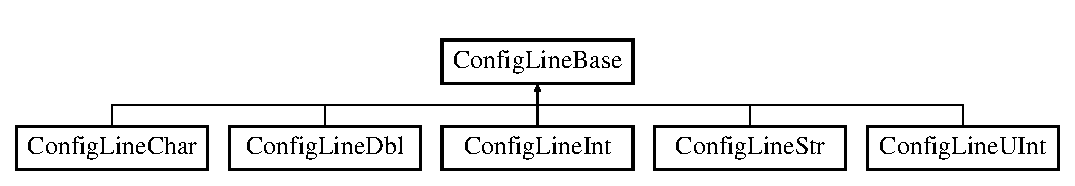
\includegraphics[height=2.000000cm]{class_config_line_base}
\end{center}
\end{figure}
\subsection*{Public Member Functions}
\begin{DoxyCompactItemize}
\item 
\mbox{\Hypertarget{class_config_line_base_acfc4ecce0bb944c4c50d87b0968df0aa}\label{class_config_line_base_acfc4ecce0bb944c4c50d87b0968df0aa}} 
std\+::string \& {\bfseries get\+Tag} ()
\item 
\mbox{\Hypertarget{class_config_line_base_ab39210affb838fa65e8dac41d7417440}\label{class_config_line_base_ab39210affb838fa65e8dac41d7417440}} 
virtual Void {\bfseries set\+Var} (std\+::string \&rc\+Value)=0
\item 
\mbox{\Hypertarget{class_config_line_base_a4ad95e64f5160e1c0ae8090b9b6d7446}\label{class_config_line_base_a4ad95e64f5160e1c0ae8090b9b6d7446}} 
virtual Void {\bfseries fprint\+Var} (F\+I\+LE $\ast$fp)=0
\end{DoxyCompactItemize}
\subsection*{Protected Member Functions}
\begin{DoxyCompactItemize}
\item 
\mbox{\Hypertarget{class_config_line_base_aeb47e5d689f562e8e120e29f6ee628a3}\label{class_config_line_base_aeb47e5d689f562e8e120e29f6ee628a3}} 
{\bfseries Config\+Line\+Base} (Char $\ast$pc\+Tag, U\+Int ui\+Type)
\end{DoxyCompactItemize}
\subsection*{Protected Attributes}
\begin{DoxyCompactItemize}
\item 
\mbox{\Hypertarget{class_config_line_base_a72648b01e5694051f91563d5e5563d14}\label{class_config_line_base_a72648b01e5694051f91563d5e5563d14}} 
std\+::string {\bfseries m\+\_\+c\+Tag}
\item 
\mbox{\Hypertarget{class_config_line_base_ae0b24b46d671b58c55756b8bfeb0092e}\label{class_config_line_base_ae0b24b46d671b58c55756b8bfeb0092e}} 
U\+Int {\bfseries m\+\_\+ui\+Type}
\end{DoxyCompactItemize}


The documentation for this class was generated from the following file\+:\begin{DoxyCompactItemize}
\item 
I\+:/\+V\+S\+R\+S4/vsrs/\+Common\+Lib\+Static/include/Parameter\+Base.\+h\end{DoxyCompactItemize}

\hypertarget{class_config_line_char}{}\section{Config\+Line\+Char Class Reference}
\label{class_config_line_char}\index{Config\+Line\+Char@{Config\+Line\+Char}}


\hyperlink{class_config_line_char}{Config\+Line\+Char} -\/ char.  




{\ttfamily \#include $<$Parameter\+Base.\+h$>$}

Inheritance diagram for Config\+Line\+Char\+:\begin{figure}[H]
\begin{center}
\leavevmode
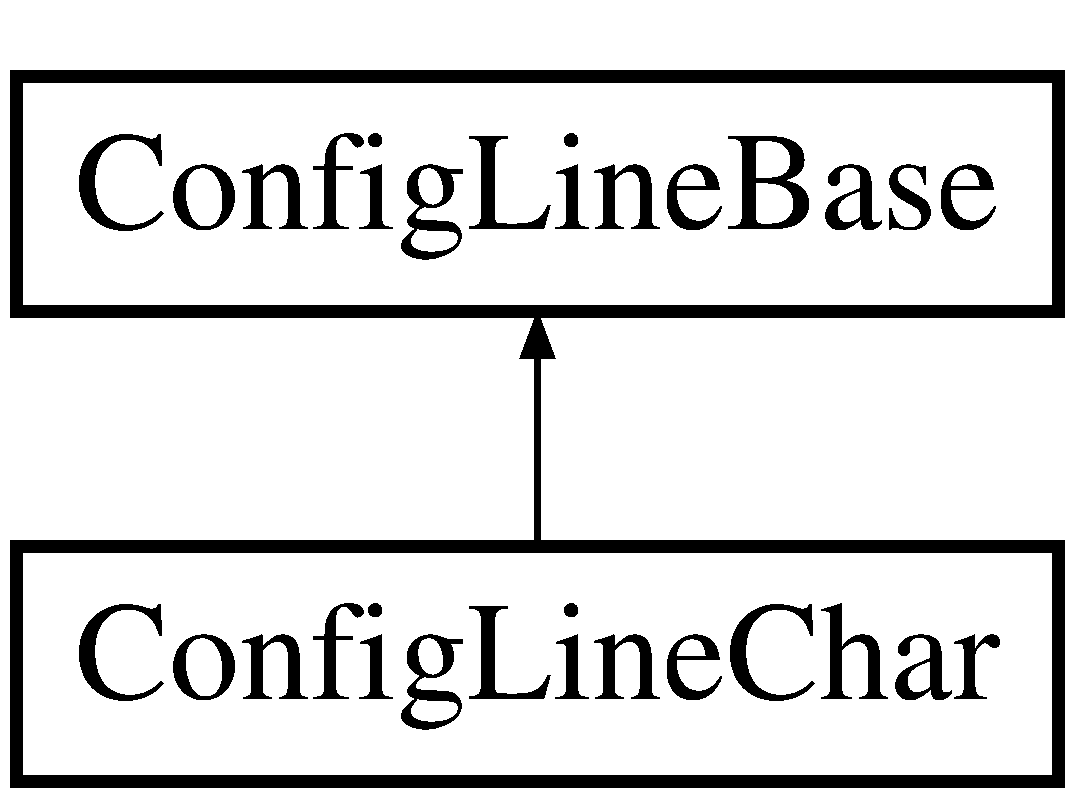
\includegraphics[height=2.000000cm]{class_config_line_char}
\end{center}
\end{figure}
\subsection*{Public Member Functions}
\begin{DoxyCompactItemize}
\item 
\mbox{\Hypertarget{class_config_line_char_a18719543fcad7ac60c01ae3fe06625fd}\label{class_config_line_char_a18719543fcad7ac60c01ae3fe06625fd}} 
{\bfseries Config\+Line\+Char} (Char $\ast$pc\+Tag, Char $\ast$pc\+Par, Char pc\+Default)
\item 
\mbox{\Hypertarget{class_config_line_char_a33253f8db8fc3e20da3aa2ba8e2e96ce}\label{class_config_line_char_a33253f8db8fc3e20da3aa2ba8e2e96ce}} 
Void {\bfseries set\+Var} (std\+::string \&pv\+Value)
\item 
\mbox{\Hypertarget{class_config_line_char_a9fb1ca4537a8c99068676f9695cb151e}\label{class_config_line_char_a9fb1ca4537a8c99068676f9695cb151e}} 
Void {\bfseries fprint\+Var} (F\+I\+LE $\ast$fp)
\end{DoxyCompactItemize}
\subsection*{Protected Attributes}
\begin{DoxyCompactItemize}
\item 
\mbox{\Hypertarget{class_config_line_char_aa8f1a92941f5ab3bcaab0f8aa852256e}\label{class_config_line_char_aa8f1a92941f5ab3bcaab0f8aa852256e}} 
Char $\ast$ {\bfseries m\+\_\+pc\+Par}
\end{DoxyCompactItemize}
\subsection*{Additional Inherited Members}


\subsection{Detailed Description}
\hyperlink{class_config_line_char}{Config\+Line\+Char} -\/ char. 

The documentation for this class was generated from the following files\+:\begin{DoxyCompactItemize}
\item 
I\+:/\+V\+S\+R\+S4/vsrs/\+Common\+Lib\+Static/include/Parameter\+Base.\+h\item 
I\+:/\+V\+S\+R\+S4/vsrs/\+Common\+Lib\+Static/src/Parameter\+Base.\+cpp\end{DoxyCompactItemize}

\hypertarget{class_config_line_dbl}{}\section{Config\+Line\+Dbl Class Reference}
\label{class_config_line_dbl}\index{Config\+Line\+Dbl@{Config\+Line\+Dbl}}


\hyperlink{class_config_line_dbl}{Config\+Line\+Dbl} -\/ double.  




{\ttfamily \#include $<$Parameter\+Base.\+h$>$}

Inheritance diagram for Config\+Line\+Dbl\+:\begin{figure}[H]
\begin{center}
\leavevmode
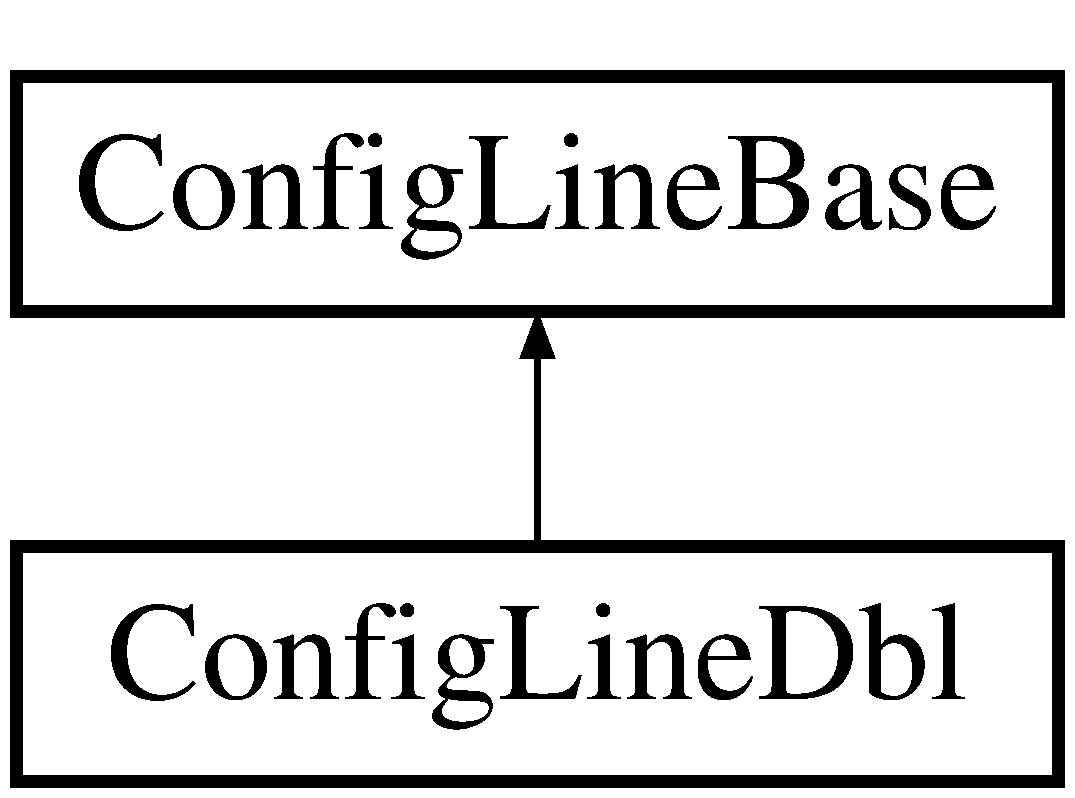
\includegraphics[height=2.000000cm]{class_config_line_dbl}
\end{center}
\end{figure}
\subsection*{Public Member Functions}
\begin{DoxyCompactItemize}
\item 
\mbox{\Hypertarget{class_config_line_dbl_aa88d87299ac96f7f98c1b7754d18994a}\label{class_config_line_dbl_aa88d87299ac96f7f98c1b7754d18994a}} 
{\bfseries Config\+Line\+Dbl} (Char $\ast$pc\+Tag, Double $\ast$pd\+Par, Double pd\+Default)
\item 
\mbox{\Hypertarget{class_config_line_dbl_aa3cdc20a68abb2f0e1707972f82e5afe}\label{class_config_line_dbl_aa3cdc20a68abb2f0e1707972f82e5afe}} 
Void {\bfseries set\+Var} (std\+::string \&pv\+Value)
\item 
\mbox{\Hypertarget{class_config_line_dbl_a98591d6e2502a0fd36f3a9c2e1c125bb}\label{class_config_line_dbl_a98591d6e2502a0fd36f3a9c2e1c125bb}} 
Void {\bfseries fprint\+Var} (F\+I\+LE $\ast$fp)
\end{DoxyCompactItemize}
\subsection*{Protected Attributes}
\begin{DoxyCompactItemize}
\item 
\mbox{\Hypertarget{class_config_line_dbl_ae39355d49a53710202359be25e1f84cc}\label{class_config_line_dbl_ae39355d49a53710202359be25e1f84cc}} 
Double $\ast$ {\bfseries m\+\_\+pd\+Par}
\end{DoxyCompactItemize}
\subsection*{Additional Inherited Members}


\subsection{Detailed Description}
\hyperlink{class_config_line_dbl}{Config\+Line\+Dbl} -\/ double. 

The documentation for this class was generated from the following files\+:\begin{DoxyCompactItemize}
\item 
I\+:/\+V\+S\+R\+S4/vsrs/\+Common\+Lib\+Static/include/Parameter\+Base.\+h\item 
I\+:/\+V\+S\+R\+S4/vsrs/\+Common\+Lib\+Static/src/Parameter\+Base.\+cpp\end{DoxyCompactItemize}

\hypertarget{class_config_line_int}{}\section{Config\+Line\+Int Class Reference}
\label{class_config_line_int}\index{Config\+Line\+Int@{Config\+Line\+Int}}


\hyperlink{class_config_line_int}{Config\+Line\+Int} -\/ int.  




{\ttfamily \#include $<$Parameter\+Base.\+h$>$}

Inheritance diagram for Config\+Line\+Int\+:\begin{figure}[H]
\begin{center}
\leavevmode
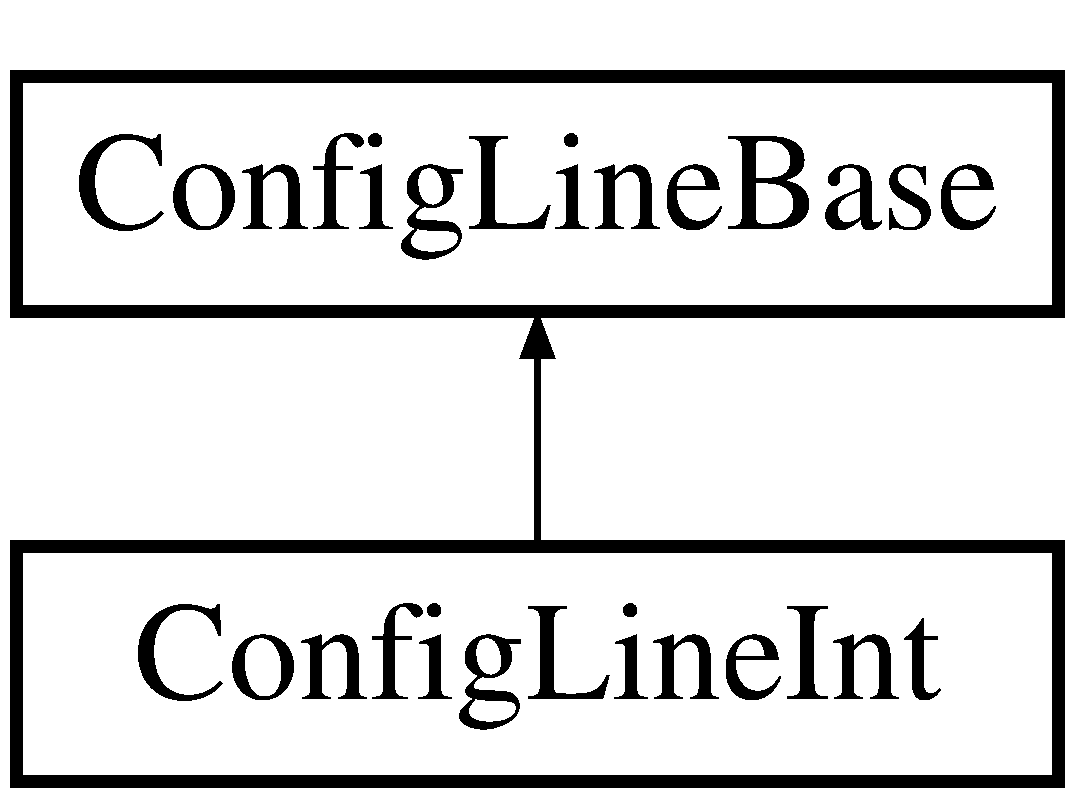
\includegraphics[height=2.000000cm]{class_config_line_int}
\end{center}
\end{figure}
\subsection*{Public Member Functions}
\begin{DoxyCompactItemize}
\item 
\mbox{\Hypertarget{class_config_line_int_a4a7466645545cb00f1282a4f3a5e9429}\label{class_config_line_int_a4a7466645545cb00f1282a4f3a5e9429}} 
{\bfseries Config\+Line\+Int} (Char $\ast$pc\+Tag, Int $\ast$pi\+Par, Int pi\+Default)
\item 
\mbox{\Hypertarget{class_config_line_int_a1d293b80d590c528ee1b801c5b995cd4}\label{class_config_line_int_a1d293b80d590c528ee1b801c5b995cd4}} 
Void {\bfseries set\+Var} (std\+::string \&pv\+Value)
\item 
\mbox{\Hypertarget{class_config_line_int_a7722943f58ef7c3ec975d4d71ece57b8}\label{class_config_line_int_a7722943f58ef7c3ec975d4d71ece57b8}} 
Void {\bfseries fprint\+Var} (F\+I\+LE $\ast$fp)
\end{DoxyCompactItemize}
\subsection*{Protected Attributes}
\begin{DoxyCompactItemize}
\item 
\mbox{\Hypertarget{class_config_line_int_ab7e7e040885db64935da23543086b8a5}\label{class_config_line_int_ab7e7e040885db64935da23543086b8a5}} 
Int $\ast$ {\bfseries m\+\_\+pi\+Par}
\end{DoxyCompactItemize}
\subsection*{Additional Inherited Members}


\subsection{Detailed Description}
\hyperlink{class_config_line_int}{Config\+Line\+Int} -\/ int. 

The documentation for this class was generated from the following files\+:\begin{DoxyCompactItemize}
\item 
I\+:/\+V\+S\+R\+S4/vsrs/\+Common\+Lib\+Static/include/Parameter\+Base.\+h\item 
I\+:/\+V\+S\+R\+S4/vsrs/\+Common\+Lib\+Static/src/Parameter\+Base.\+cpp\end{DoxyCompactItemize}

\hypertarget{class_config_line_str}{}\section{Config\+Line\+Str Class Reference}
\label{class_config_line_str}\index{Config\+Line\+Str@{Config\+Line\+Str}}


\hyperlink{class_config_line_str}{Config\+Line\+Str} -\/ string.  




{\ttfamily \#include $<$Parameter\+Base.\+h$>$}

Inheritance diagram for Config\+Line\+Str\+:\begin{figure}[H]
\begin{center}
\leavevmode
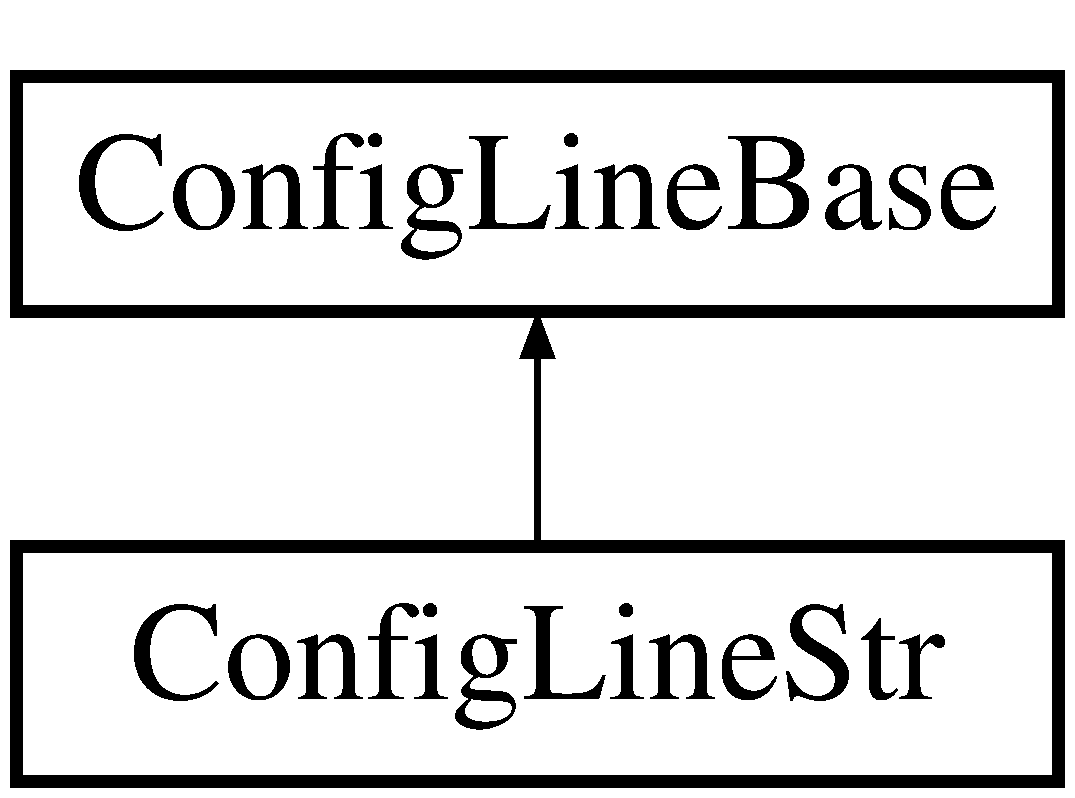
\includegraphics[height=2.000000cm]{class_config_line_str}
\end{center}
\end{figure}
\subsection*{Public Member Functions}
\begin{DoxyCompactItemize}
\item 
\mbox{\Hypertarget{class_config_line_str_a0d78882f2ce3e7474aff5a39677a706a}\label{class_config_line_str_a0d78882f2ce3e7474aff5a39677a706a}} 
{\bfseries Config\+Line\+Str} (Char $\ast$pc\+Tag, std\+::string $\ast$pc\+Par, Char $\ast$pc\+Default)
\item 
\mbox{\Hypertarget{class_config_line_str_a513b0f223d8ee74863c03c0e4741968c}\label{class_config_line_str_a513b0f223d8ee74863c03c0e4741968c}} 
Void {\bfseries set\+Var} (std\+::string \&pv\+Value)
\item 
\mbox{\Hypertarget{class_config_line_str_a0356b0e3f2e7fef3e290f4eb7b1950d6}\label{class_config_line_str_a0356b0e3f2e7fef3e290f4eb7b1950d6}} 
Void {\bfseries fprint\+Var} (F\+I\+LE $\ast$fp)
\end{DoxyCompactItemize}
\subsection*{Protected Attributes}
\begin{DoxyCompactItemize}
\item 
\mbox{\Hypertarget{class_config_line_str_acac7a95f4ae1e49073b689743e5175cd}\label{class_config_line_str_acac7a95f4ae1e49073b689743e5175cd}} 
std\+::string $\ast$ {\bfseries m\+\_\+pc\+Par}
\end{DoxyCompactItemize}
\subsection*{Additional Inherited Members}


\subsection{Detailed Description}
\hyperlink{class_config_line_str}{Config\+Line\+Str} -\/ string. 

The documentation for this class was generated from the following files\+:\begin{DoxyCompactItemize}
\item 
I\+:/\+V\+S\+R\+S4/vsrs/\+Common\+Lib\+Static/include/Parameter\+Base.\+h\item 
I\+:/\+V\+S\+R\+S4/vsrs/\+Common\+Lib\+Static/src/Parameter\+Base.\+cpp\end{DoxyCompactItemize}

\hypertarget{class_config_line_u_int}{}\section{Config\+Line\+U\+Int Class Reference}
\label{class_config_line_u_int}\index{Config\+Line\+U\+Int@{Config\+Line\+U\+Int}}


\hyperlink{class_config_line_u_int}{Config\+Line\+U\+Int} -\/ uint.  




{\ttfamily \#include $<$Parameter\+Base.\+h$>$}

Inheritance diagram for Config\+Line\+U\+Int\+:\begin{figure}[H]
\begin{center}
\leavevmode
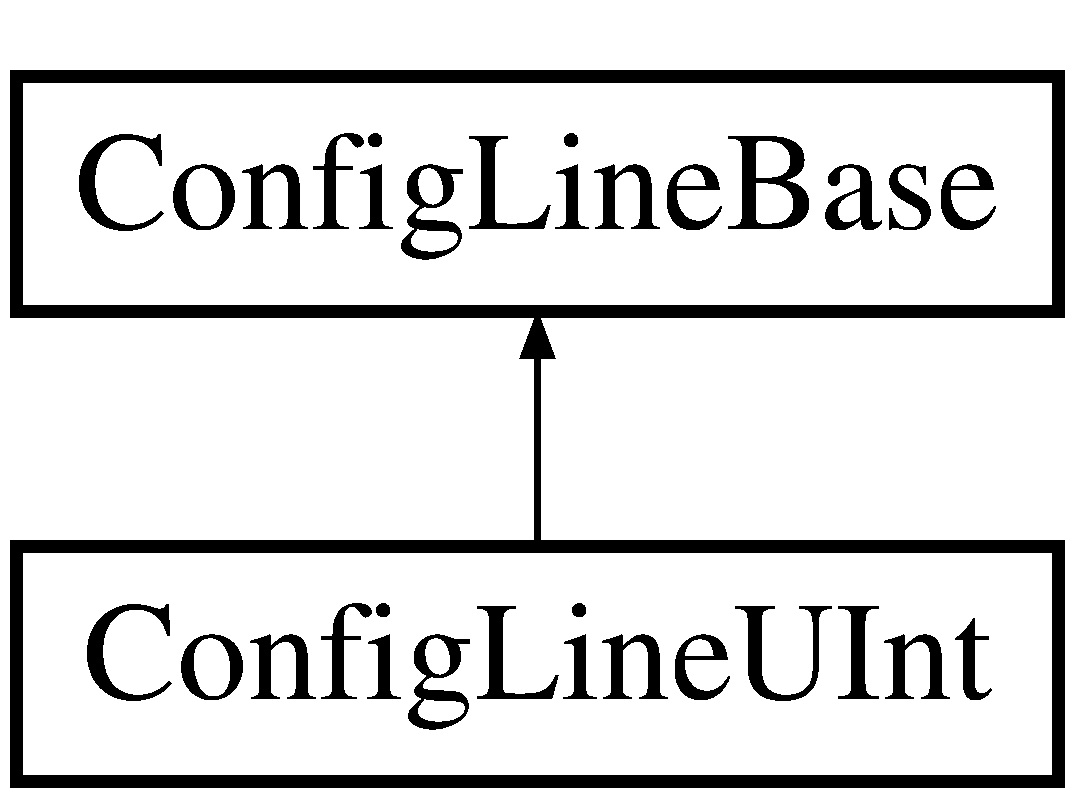
\includegraphics[height=2.000000cm]{class_config_line_u_int}
\end{center}
\end{figure}
\subsection*{Public Member Functions}
\begin{DoxyCompactItemize}
\item 
\mbox{\Hypertarget{class_config_line_u_int_acb0d037599b6447947678c85fad975ee}\label{class_config_line_u_int_acb0d037599b6447947678c85fad975ee}} 
{\bfseries Config\+Line\+U\+Int} (Char $\ast$pc\+Tag, U\+Int $\ast$pui\+Par, U\+Int pui\+Default)
\item 
\mbox{\Hypertarget{class_config_line_u_int_a1cd46e08503002f9e76ac38520d885ae}\label{class_config_line_u_int_a1cd46e08503002f9e76ac38520d885ae}} 
Void {\bfseries set\+Var} (std\+::string \&pv\+Value)
\item 
\mbox{\Hypertarget{class_config_line_u_int_a4d2d13d31eb3f66465486e3abea8bf02}\label{class_config_line_u_int_a4d2d13d31eb3f66465486e3abea8bf02}} 
Void {\bfseries fprint\+Var} (F\+I\+LE $\ast$fp)
\end{DoxyCompactItemize}
\subsection*{Protected Attributes}
\begin{DoxyCompactItemize}
\item 
\mbox{\Hypertarget{class_config_line_u_int_a865997c21f034ad3a942f8701763bedd}\label{class_config_line_u_int_a865997c21f034ad3a942f8701763bedd}} 
U\+Int $\ast$ {\bfseries m\+\_\+pui\+Par}
\end{DoxyCompactItemize}
\subsection*{Additional Inherited Members}


\subsection{Detailed Description}
\hyperlink{class_config_line_u_int}{Config\+Line\+U\+Int} -\/ uint. 

The documentation for this class was generated from the following files\+:\begin{DoxyCompactItemize}
\item 
I\+:/\+V\+S\+R\+S4/vsrs/\+Common\+Lib\+Static/include/Parameter\+Base.\+h\item 
I\+:/\+V\+S\+R\+S4/vsrs/\+Common\+Lib\+Static/src/Parameter\+Base.\+cpp\end{DoxyCompactItemize}

\hypertarget{class_c_parameter_view_interpolation}{}\section{C\+Parameter\+View\+Interpolation Class Reference}
\label{class_c_parameter_view_interpolation}\index{C\+Parameter\+View\+Interpolation@{C\+Parameter\+View\+Interpolation}}
Inheritance diagram for C\+Parameter\+View\+Interpolation\+:\begin{figure}[H]
\begin{center}
\leavevmode
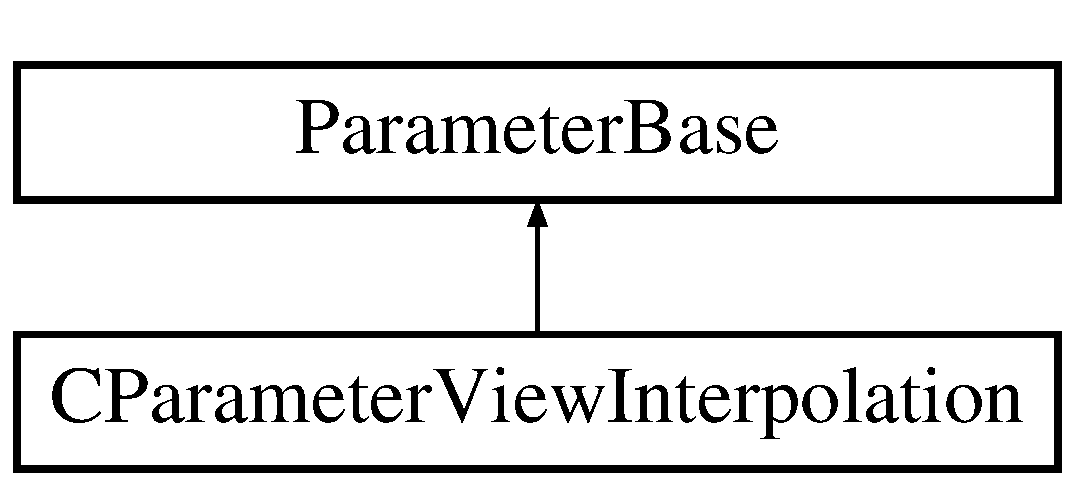
\includegraphics[height=2.000000cm]{class_c_parameter_view_interpolation}
\end{center}
\end{figure}
\subsection*{Public Member Functions}
\begin{DoxyCompactItemize}
\item 
\mbox{\Hypertarget{class_c_parameter_view_interpolation_a961db258894c7565cbd96b4139862202}\label{class_c_parameter_view_interpolation_a961db258894c7565cbd96b4139862202}} 
Int {\bfseries Init} (Int argc, Char $\ast$$\ast$argv)
\item 
\mbox{\Hypertarget{class_c_parameter_view_interpolation_a7ace89f8820f5cf8d3737346e894aec2}\label{class_c_parameter_view_interpolation_a7ace89f8820f5cf8d3737346e894aec2}} 
Void {\bfseries set\+Depth\+Type} (U\+Int ui)
\item 
\mbox{\Hypertarget{class_c_parameter_view_interpolation_a8238f75280c8f88e4cfef138e9536b2c}\label{class_c_parameter_view_interpolation_a8238f75280c8f88e4cfef138e9536b2c}} 
Void {\bfseries set\+Source\+Width} (U\+Int ui)
\item 
\mbox{\Hypertarget{class_c_parameter_view_interpolation_ad8ba940b4b46342f873af9b43ca3a416}\label{class_c_parameter_view_interpolation_ad8ba940b4b46342f873af9b43ca3a416}} 
Void {\bfseries set\+Source\+Height} (U\+Int ui)
\item 
\mbox{\Hypertarget{class_c_parameter_view_interpolation_a89cbf09896d476daa071086a77f2928f}\label{class_c_parameter_view_interpolation_a89cbf09896d476daa071086a77f2928f}} 
Void {\bfseries set\+Number\+Of\+Frames} (U\+Int ui)
\item 
\mbox{\Hypertarget{class_c_parameter_view_interpolation_a224e7637c9674f3c0e25856e7fe95273}\label{class_c_parameter_view_interpolation_a224e7637c9674f3c0e25856e7fe95273}} 
Void {\bfseries set\+Start\+Frame} (U\+Int ui)
\item 
\mbox{\Hypertarget{class_c_parameter_view_interpolation_a94cd514abb5a2edf388364f355943660}\label{class_c_parameter_view_interpolation_a94cd514abb5a2edf388364f355943660}} 
Void {\bfseries set\+Left\+Nearest\+Depth\+Value} (Double d)
\item 
\mbox{\Hypertarget{class_c_parameter_view_interpolation_a0865afd4135d955227e0d51d2f8fea38}\label{class_c_parameter_view_interpolation_a0865afd4135d955227e0d51d2f8fea38}} 
Void {\bfseries set\+Left\+Farthest\+Depth\+Value} (Double d)
\item 
\mbox{\Hypertarget{class_c_parameter_view_interpolation_a766501036e92be9537176ab1df6b186a}\label{class_c_parameter_view_interpolation_a766501036e92be9537176ab1df6b186a}} 
Void {\bfseries set\+Right\+Nearest\+Depth\+Value} (Double d)
\item 
\mbox{\Hypertarget{class_c_parameter_view_interpolation_a6a9b646b572cc5638c6118d0244928ee}\label{class_c_parameter_view_interpolation_a6a9b646b572cc5638c6118d0244928ee}} 
Void {\bfseries set\+Right\+Farthest\+Depth\+Value} (Double d)
\item 
\mbox{\Hypertarget{class_c_parameter_view_interpolation_a57294252442087a252e9c4b2df17329d}\label{class_c_parameter_view_interpolation_a57294252442087a252e9c4b2df17329d}} 
Void {\bfseries set\+Camera\+Parameter\+File} (std\+::string s)
\item 
\mbox{\Hypertarget{class_c_parameter_view_interpolation_a4849b8a51c0b692a228a3b58c3dada63}\label{class_c_parameter_view_interpolation_a4849b8a51c0b692a228a3b58c3dada63}} 
Void {\bfseries set\+Left\+Camera\+Name} (std\+::string s)
\item 
\mbox{\Hypertarget{class_c_parameter_view_interpolation_a836d334cfa4a2b58bd9118e0e17c4def}\label{class_c_parameter_view_interpolation_a836d334cfa4a2b58bd9118e0e17c4def}} 
Void {\bfseries set\+Virtual\+Camera\+Name} (std\+::string s)
\item 
\mbox{\Hypertarget{class_c_parameter_view_interpolation_af3754eeb38b7e6c8612cc0716f1f62ed}\label{class_c_parameter_view_interpolation_af3754eeb38b7e6c8612cc0716f1f62ed}} 
Void {\bfseries set\+Right\+Camera\+Name} (std\+::string s)
\item 
\mbox{\Hypertarget{class_c_parameter_view_interpolation_a678892902823f4fbdb28ccbbf5f9c665}\label{class_c_parameter_view_interpolation_a678892902823f4fbdb28ccbbf5f9c665}} 
Void {\bfseries set\+Left\+View\+Image\+Name} (std\+::string s)
\item 
\mbox{\Hypertarget{class_c_parameter_view_interpolation_a71852478879599e5093597ed7c7e2c05}\label{class_c_parameter_view_interpolation_a71852478879599e5093597ed7c7e2c05}} 
Void {\bfseries set\+Right\+View\+Image\+Name} (std\+::string s)
\item 
\mbox{\Hypertarget{class_c_parameter_view_interpolation_aee3b6b4d5a5c01a364cc04bd1a27d073}\label{class_c_parameter_view_interpolation_aee3b6b4d5a5c01a364cc04bd1a27d073}} 
Void {\bfseries set\+Left\+Depth\+Map\+Name} (std\+::string s)
\item 
\mbox{\Hypertarget{class_c_parameter_view_interpolation_ae2e7d0f67c99e3f0ceae6c7ea045d99f}\label{class_c_parameter_view_interpolation_ae2e7d0f67c99e3f0ceae6c7ea045d99f}} 
Void {\bfseries set\+Right\+Depth\+Map\+Name} (std\+::string s)
\item 
\mbox{\Hypertarget{class_c_parameter_view_interpolation_a61aeccf88f9866bbed5b272b2e1ef7ad}\label{class_c_parameter_view_interpolation_a61aeccf88f9866bbed5b272b2e1ef7ad}} 
Void {\bfseries set\+Output\+Vir\+View\+Image\+Name} (std\+::string s)
\item 
\mbox{\Hypertarget{class_c_parameter_view_interpolation_a1a86e2216a7879a7913651aa16091fc7}\label{class_c_parameter_view_interpolation_a1a86e2216a7879a7913651aa16091fc7}} 
Void {\bfseries set\+Color\+Space} (U\+Int ui)
\item 
\mbox{\Hypertarget{class_c_parameter_view_interpolation_a60b41d616b6741df710e3677b56f7ccf}\label{class_c_parameter_view_interpolation_a60b41d616b6741df710e3677b56f7ccf}} 
Void {\bfseries set\+Precision} (U\+Int ui)
\item 
\mbox{\Hypertarget{class_c_parameter_view_interpolation_a64efaf0447f861af573e77a4b4875da0}\label{class_c_parameter_view_interpolation_a64efaf0447f861af573e77a4b4875da0}} 
Void {\bfseries set\+Filter} (U\+Int ui)
\item 
\mbox{\Hypertarget{class_c_parameter_view_interpolation_ab06ad375f761b79db3ae85531a9f6eef}\label{class_c_parameter_view_interpolation_ab06ad375f761b79db3ae85531a9f6eef}} 
Void {\bfseries set\+Ivsrs\+Inpaint} (U\+Int ui)
\item 
\mbox{\Hypertarget{class_c_parameter_view_interpolation_a2657339e853b43b68ac453bf43f92af8}\label{class_c_parameter_view_interpolation_a2657339e853b43b68ac453bf43f92af8}} 
Void {\bfseries set\+Synthesis\+Mode} (U\+Int ui)
\item 
\mbox{\Hypertarget{class_c_parameter_view_interpolation_adb3c34864ade04d8715ec29f08627bd1}\label{class_c_parameter_view_interpolation_adb3c34864ade04d8715ec29f08627bd1}} 
U\+Int {\bfseries set\+Boundary\+Noise\+Removal} (U\+Int ui)
\item 
\mbox{\Hypertarget{class_c_parameter_view_interpolation_a534045083053e8375b523124880ebbe5}\label{class_c_parameter_view_interpolation_a534045083053e8375b523124880ebbe5}} 
Void {\bfseries set\+View\+Blending} (U\+Int ui)
\item 
\mbox{\Hypertarget{class_c_parameter_view_interpolation_a1f7d96718183a3aed5c1c04548150af7}\label{class_c_parameter_view_interpolation_a1f7d96718183a3aed5c1c04548150af7}} 
Void {\bfseries set\+Depth\+Blend\+Diff} (Int i)
\item 
\mbox{\Hypertarget{class_c_parameter_view_interpolation_ac3c62a0e0a17610adb933bc48b0449dd}\label{class_c_parameter_view_interpolation_ac3c62a0e0a17610adb933bc48b0449dd}} 
U\+Int {\bfseries get\+Depth\+Type} ()
\item 
\mbox{\Hypertarget{class_c_parameter_view_interpolation_af1f1efe5ada2c7d0f5b7adbd9d236364}\label{class_c_parameter_view_interpolation_af1f1efe5ada2c7d0f5b7adbd9d236364}} 
U\+Int {\bfseries get\+Source\+Width} ()
\item 
\mbox{\Hypertarget{class_c_parameter_view_interpolation_aad1e0667662870e6ef46cf14cf21ce56}\label{class_c_parameter_view_interpolation_aad1e0667662870e6ef46cf14cf21ce56}} 
U\+Int {\bfseries get\+Source\+Height} ()
\item 
\mbox{\Hypertarget{class_c_parameter_view_interpolation_ab883803b39e96cdd77dd0f1f0d277cfc}\label{class_c_parameter_view_interpolation_ab883803b39e96cdd77dd0f1f0d277cfc}} 
U\+Int {\bfseries get\+Number\+Of\+Frames} ()
\item 
\mbox{\Hypertarget{class_c_parameter_view_interpolation_ad31442ae319f0443e03977c10b96f30b}\label{class_c_parameter_view_interpolation_ad31442ae319f0443e03977c10b96f30b}} 
U\+Int {\bfseries get\+Start\+Frame} ()
\item 
\mbox{\Hypertarget{class_c_parameter_view_interpolation_ab09927c7c726c08e7f30e9d64f844ff6}\label{class_c_parameter_view_interpolation_ab09927c7c726c08e7f30e9d64f844ff6}} 
Double {\bfseries get\+Left\+Nearest\+Depth\+Value} ()
\item 
\mbox{\Hypertarget{class_c_parameter_view_interpolation_a90971cab7323c128a4c1bcbe81c53298}\label{class_c_parameter_view_interpolation_a90971cab7323c128a4c1bcbe81c53298}} 
Double {\bfseries get\+Left\+Farthest\+Depth\+Value} ()
\item 
\mbox{\Hypertarget{class_c_parameter_view_interpolation_a30dcb60c7c62367161cc299c0b286da0}\label{class_c_parameter_view_interpolation_a30dcb60c7c62367161cc299c0b286da0}} 
Double {\bfseries get\+Right\+Nearest\+Depth\+Value} ()
\item 
\mbox{\Hypertarget{class_c_parameter_view_interpolation_a799a87e7f0af476ee583a305bc0cc4ad}\label{class_c_parameter_view_interpolation_a799a87e7f0af476ee583a305bc0cc4ad}} 
Double {\bfseries get\+Right\+Farthest\+Depth\+Value} ()
\item 
\mbox{\Hypertarget{class_c_parameter_view_interpolation_adc2dff565cccbf6ccff56d94940a1059}\label{class_c_parameter_view_interpolation_adc2dff565cccbf6ccff56d94940a1059}} 
const std\+::string {\bfseries get\+Camera\+Parameter\+File} ()
\item 
\mbox{\Hypertarget{class_c_parameter_view_interpolation_af032780f8ae6780b337ccb6940d96834}\label{class_c_parameter_view_interpolation_af032780f8ae6780b337ccb6940d96834}} 
const std\+::string {\bfseries get\+Left\+Camera\+Name} ()
\item 
\mbox{\Hypertarget{class_c_parameter_view_interpolation_af69530b3e2be33cc97eb6a79692db5b1}\label{class_c_parameter_view_interpolation_af69530b3e2be33cc97eb6a79692db5b1}} 
const std\+::string {\bfseries get\+Virtual\+Camera\+Name} ()
\item 
\mbox{\Hypertarget{class_c_parameter_view_interpolation_a1093545d9864d93dfd21967658fd5afa}\label{class_c_parameter_view_interpolation_a1093545d9864d93dfd21967658fd5afa}} 
const std\+::string {\bfseries get\+Right\+Camera\+Name} ()
\item 
\mbox{\Hypertarget{class_c_parameter_view_interpolation_a8d1d4b59ef902fec6c5f43c3ef2d05bc}\label{class_c_parameter_view_interpolation_a8d1d4b59ef902fec6c5f43c3ef2d05bc}} 
const std\+::string {\bfseries get\+Left\+View\+Image\+Name} ()
\item 
\mbox{\Hypertarget{class_c_parameter_view_interpolation_a501ed70a5f7415cbd7748ca8070bcd3a}\label{class_c_parameter_view_interpolation_a501ed70a5f7415cbd7748ca8070bcd3a}} 
const std\+::string {\bfseries get\+Right\+View\+Image\+Name} ()
\item 
\mbox{\Hypertarget{class_c_parameter_view_interpolation_ac803144844b2e210940f7cb673a7b159}\label{class_c_parameter_view_interpolation_ac803144844b2e210940f7cb673a7b159}} 
const std\+::string {\bfseries get\+Left\+Depth\+Map\+Name} ()
\item 
\mbox{\Hypertarget{class_c_parameter_view_interpolation_a89194b315ad977b009878ee3b406b6ff}\label{class_c_parameter_view_interpolation_a89194b315ad977b009878ee3b406b6ff}} 
const std\+::string {\bfseries get\+Right\+Depth\+Map\+Name} ()
\item 
\mbox{\Hypertarget{class_c_parameter_view_interpolation_a9f6aa65acc511a41dcb1b3ef06a94d33}\label{class_c_parameter_view_interpolation_a9f6aa65acc511a41dcb1b3ef06a94d33}} 
const std\+::string {\bfseries get\+Output\+Vir\+View\+Image\+Name} ()
\item 
\mbox{\Hypertarget{class_c_parameter_view_interpolation_ad3be9eaafe1247fe1c4bd31ac98425db}\label{class_c_parameter_view_interpolation_ad3be9eaafe1247fe1c4bd31ac98425db}} 
Double {\bfseries get\+Focal\+Length} ()
\item 
\mbox{\Hypertarget{class_c_parameter_view_interpolation_a387cb9dcf222916b3b10597870f798a8}\label{class_c_parameter_view_interpolation_a387cb9dcf222916b3b10597870f798a8}} 
Double {\bfseries get\+L\+Translation\+Left} ()
\item 
\mbox{\Hypertarget{class_c_parameter_view_interpolation_ac981cd52e55a634a61689467c6bf5f95}\label{class_c_parameter_view_interpolation_ac981cd52e55a634a61689467c6bf5f95}} 
Double {\bfseries get\+L\+Translation\+Right} ()
\item 
\mbox{\Hypertarget{class_c_parameter_view_interpolation_a1e8781654145eb710000592a7110ed5d}\label{class_c_parameter_view_interpolation_a1e8781654145eb710000592a7110ed5d}} 
Double {\bfseries getdu\+Principal\+Left} ()
\item 
\mbox{\Hypertarget{class_c_parameter_view_interpolation_a18d8a21c14197800306131e2600b6009}\label{class_c_parameter_view_interpolation_a18d8a21c14197800306131e2600b6009}} 
Double {\bfseries getdu\+Principal\+Right} ()
\item 
\mbox{\Hypertarget{class_c_parameter_view_interpolation_a32a50c8e6d51e82a51b8e0495a5c0783}\label{class_c_parameter_view_interpolation_a32a50c8e6d51e82a51b8e0495a5c0783}} 
Double $\ast$ {\bfseries get\+Mat\+\_\+\+Ex\+\_\+\+Left} ()
\item 
\mbox{\Hypertarget{class_c_parameter_view_interpolation_a0e570da1cc6019996ed22220e0403c09}\label{class_c_parameter_view_interpolation_a0e570da1cc6019996ed22220e0403c09}} 
Double $\ast$ {\bfseries get\+Mat\+\_\+\+Ex\+\_\+\+Virtual} ()
\item 
\mbox{\Hypertarget{class_c_parameter_view_interpolation_a6f7fe7b27b5012046d56d67bdf1ab242}\label{class_c_parameter_view_interpolation_a6f7fe7b27b5012046d56d67bdf1ab242}} 
Double $\ast$ {\bfseries get\+Mat\+\_\+\+Ex\+\_\+\+Right} ()
\item 
\mbox{\Hypertarget{class_c_parameter_view_interpolation_a1d5f103f56a0907661ad575a9b6d5f9e}\label{class_c_parameter_view_interpolation_a1d5f103f56a0907661ad575a9b6d5f9e}} 
Double $\ast$ {\bfseries get\+Mat\+\_\+\+In\+\_\+\+Left} ()
\item 
\mbox{\Hypertarget{class_c_parameter_view_interpolation_ad06e08be882ef12cd85e7366d515d83b}\label{class_c_parameter_view_interpolation_ad06e08be882ef12cd85e7366d515d83b}} 
Double $\ast$ {\bfseries get\+Mat\+\_\+\+In\+\_\+\+Virtual} ()
\item 
\mbox{\Hypertarget{class_c_parameter_view_interpolation_a4318619b0bcb86e66ad291c54bcca94f}\label{class_c_parameter_view_interpolation_a4318619b0bcb86e66ad291c54bcca94f}} 
Double $\ast$ {\bfseries get\+Mat\+\_\+\+In\+\_\+\+Right} ()
\item 
\mbox{\Hypertarget{class_c_parameter_view_interpolation_a259482cc9b41e6f0e5c8312ad050f487}\label{class_c_parameter_view_interpolation_a259482cc9b41e6f0e5c8312ad050f487}} 
Double $\ast$ {\bfseries get\+Mat\+\_\+\+Trans\+\_\+\+Left} ()
\item 
\mbox{\Hypertarget{class_c_parameter_view_interpolation_abc4d30777d00a4c6081ddf2e786326b7}\label{class_c_parameter_view_interpolation_abc4d30777d00a4c6081ddf2e786326b7}} 
Double $\ast$ {\bfseries get\+Mat\+\_\+\+Trans\+\_\+\+Virtual} ()
\item 
\mbox{\Hypertarget{class_c_parameter_view_interpolation_ad5f57642f28db5436c336a0a4149613d}\label{class_c_parameter_view_interpolation_ad5f57642f28db5436c336a0a4149613d}} 
Double $\ast$ {\bfseries get\+Mat\+\_\+\+Trans\+\_\+\+Right} ()
\item 
\mbox{\Hypertarget{class_c_parameter_view_interpolation_a8a14394928eaa20ef7bcb56f06cda8f6}\label{class_c_parameter_view_interpolation_a8a14394928eaa20ef7bcb56f06cda8f6}} 
Double {\bfseries get\+Left\+Baseline\+Distance} ()
\item 
\mbox{\Hypertarget{class_c_parameter_view_interpolation_a6c0fc0a080c8c115d71bd958732da8a0}\label{class_c_parameter_view_interpolation_a6c0fc0a080c8c115d71bd958732da8a0}} 
Double {\bfseries get\+Right\+Baseline\+Distance} ()
\item 
\mbox{\Hypertarget{class_c_parameter_view_interpolation_a34da9342cdaba7a113a3395bf0b00cf3}\label{class_c_parameter_view_interpolation_a34da9342cdaba7a113a3395bf0b00cf3}} 
Int {\bfseries get\+Splatting\+Option} ()
\item 
\mbox{\Hypertarget{class_c_parameter_view_interpolation_aac0d2baf0d17999732762582c4e65f81}\label{class_c_parameter_view_interpolation_aac0d2baf0d17999732762582c4e65f81}} 
Int {\bfseries get\+Boudary\+Growth} ()
\item 
\mbox{\Hypertarget{class_c_parameter_view_interpolation_a31d10722be924d455928783ec4f7c455}\label{class_c_parameter_view_interpolation_a31d10722be924d455928783ec4f7c455}} 
Int {\bfseries get\+Merging\+Option} ()
\item 
\mbox{\Hypertarget{class_c_parameter_view_interpolation_a771c8d2fc5ec1c635b401b293ed6e67a}\label{class_c_parameter_view_interpolation_a771c8d2fc5ec1c635b401b293ed6e67a}} 
Int {\bfseries get\+Depth\+Threshold} ()
\item 
\mbox{\Hypertarget{class_c_parameter_view_interpolation_ac75ee184493afa4f3175036ce94943d0}\label{class_c_parameter_view_interpolation_ac75ee184493afa4f3175036ce94943d0}} 
Int {\bfseries get\+Hole\+Count\+Threshold} ()
\item 
\mbox{\Hypertarget{class_c_parameter_view_interpolation_a395782e8c923c44892c1239247b57b7d}\label{class_c_parameter_view_interpolation_a395782e8c923c44892c1239247b57b7d}} 
Int {\bfseries get\+Temporal\+Improvement\+Option} ()
\item 
\mbox{\Hypertarget{class_c_parameter_view_interpolation_aa1907263396ba876a05c18b00a8e7adb}\label{class_c_parameter_view_interpolation_aa1907263396ba876a05c18b00a8e7adb}} 
Int {\bfseries get\+Warp\+Enhancement\+Option} ()
\item 
\mbox{\Hypertarget{class_c_parameter_view_interpolation_ae9b854cc0b1e609c977bebd429cf232a}\label{class_c_parameter_view_interpolation_ae9b854cc0b1e609c977bebd429cf232a}} 
Int {\bfseries get\+Clean\+Noise\+Option} ()
\item 
\mbox{\Hypertarget{class_c_parameter_view_interpolation_a85e6428b77c01977ce5ac1ef46cf125d}\label{class_c_parameter_view_interpolation_a85e6428b77c01977ce5ac1ef46cf125d}} 
U\+Int {\bfseries get\+Color\+Space} ()
\item 
\mbox{\Hypertarget{class_c_parameter_view_interpolation_a9b6fdecd102b9c150bd57f48d1438b4d}\label{class_c_parameter_view_interpolation_a9b6fdecd102b9c150bd57f48d1438b4d}} 
U\+Int {\bfseries get\+Precision} ()
\item 
\mbox{\Hypertarget{class_c_parameter_view_interpolation_a58d04a3c19769ce85fccc1e50c6e8526}\label{class_c_parameter_view_interpolation_a58d04a3c19769ce85fccc1e50c6e8526}} 
U\+Int {\bfseries get\+Filter} ()
\item 
\mbox{\Hypertarget{class_c_parameter_view_interpolation_ac90fbcd7fc1406384b0b32ac64f2b41e}\label{class_c_parameter_view_interpolation_ac90fbcd7fc1406384b0b32ac64f2b41e}} 
U\+Int {\bfseries get\+Ivsrs\+Inpaint} ()
\item 
\mbox{\Hypertarget{class_c_parameter_view_interpolation_a0d8c47b6bb4b852d11fe4c8a2a11ffb4}\label{class_c_parameter_view_interpolation_a0d8c47b6bb4b852d11fe4c8a2a11ffb4}} 
U\+Int {\bfseries get\+Synthesis\+Mode} ()
\item 
\mbox{\Hypertarget{class_c_parameter_view_interpolation_adbf182c15b3b7428e82ef3ceb69f75be}\label{class_c_parameter_view_interpolation_adbf182c15b3b7428e82ef3ceb69f75be}} 
U\+Int {\bfseries get\+Boundary\+Noise\+Removal} ()
\item 
\mbox{\Hypertarget{class_c_parameter_view_interpolation_ad52c94371d4bedf276982204a81fcd14}\label{class_c_parameter_view_interpolation_ad52c94371d4bedf276982204a81fcd14}} 
U\+Int {\bfseries get\+View\+Blending} ()
\item 
\mbox{\Hypertarget{class_c_parameter_view_interpolation_a903c9c8e4dd2108815b15c24d16a7646}\label{class_c_parameter_view_interpolation_a903c9c8e4dd2108815b15c24d16a7646}} 
Int {\bfseries get\+Depth\+Blend\+Diff} ()
\end{DoxyCompactItemize}
\subsection*{Protected Member Functions}
\begin{DoxyCompactItemize}
\item 
\mbox{\Hypertarget{class_c_parameter_view_interpolation_a92a566cd47c6373ada412b7390a63d24}\label{class_c_parameter_view_interpolation_a92a566cd47c6373ada412b7390a63d24}} 
Int {\bfseries x\+Print\+Usage} (Char $\ast$$\ast$argv)
\end{DoxyCompactItemize}
\subsection*{Protected Attributes}
\begin{DoxyCompactItemize}
\item 
U\+Int \hyperlink{class_c_parameter_view_interpolation_ad129c82c944146c2433758a88671acef}{m\+\_\+ui\+Depth\+Type}
\item 
\mbox{\Hypertarget{class_c_parameter_view_interpolation_abad31f5db95ef3bc590bb7d3ba62290b}\label{class_c_parameter_view_interpolation_abad31f5db95ef3bc590bb7d3ba62290b}} 
U\+Int \hyperlink{class_c_parameter_view_interpolation_abad31f5db95ef3bc590bb7d3ba62290b}{m\+\_\+ui\+Source\+Width}
\begin{DoxyCompactList}\small\item\em Input frame width. Default\+: 0. \end{DoxyCompactList}\item 
\mbox{\Hypertarget{class_c_parameter_view_interpolation_a204bc8d1c5630f4de4bbcb93bcf70676}\label{class_c_parameter_view_interpolation_a204bc8d1c5630f4de4bbcb93bcf70676}} 
U\+Int \hyperlink{class_c_parameter_view_interpolation_a204bc8d1c5630f4de4bbcb93bcf70676}{m\+\_\+ui\+Source\+Height}
\begin{DoxyCompactList}\small\item\em Input frame height. Default\+: 0. \end{DoxyCompactList}\item 
\mbox{\Hypertarget{class_c_parameter_view_interpolation_abd8e092068896fc0ff436c7033bf1300}\label{class_c_parameter_view_interpolation_abd8e092068896fc0ff436c7033bf1300}} 
U\+Int \hyperlink{class_c_parameter_view_interpolation_abd8e092068896fc0ff436c7033bf1300}{m\+\_\+ui\+Number\+Of\+Frames}
\begin{DoxyCompactList}\small\item\em Total number of input frame. Default\+: 0. \end{DoxyCompactList}\item 
\mbox{\Hypertarget{class_c_parameter_view_interpolation_a8d5713730b3f7271598bf00d986f9efe}\label{class_c_parameter_view_interpolation_a8d5713730b3f7271598bf00d986f9efe}} 
U\+Int \hyperlink{class_c_parameter_view_interpolation_a8d5713730b3f7271598bf00d986f9efe}{m\+\_\+ui\+Start\+Frame}
\begin{DoxyCompactList}\small\item\em Starting frame \#. Default\+: 0. \end{DoxyCompactList}\item 
\mbox{\Hypertarget{class_c_parameter_view_interpolation_afa4540ab1a006b8922471f97d36fb510}\label{class_c_parameter_view_interpolation_afa4540ab1a006b8922471f97d36fb510}} 
Double \hyperlink{class_c_parameter_view_interpolation_afa4540ab1a006b8922471f97d36fb510}{m\+\_\+d\+Left\+Nearest\+Depth\+Value}
\begin{DoxyCompactList}\small\item\em Nearest depth value of left image from camera or the origin of 3D space. Default\+: 0. \end{DoxyCompactList}\item 
\mbox{\Hypertarget{class_c_parameter_view_interpolation_a3faa42553cfa75f1ea31489d2b35d6f8}\label{class_c_parameter_view_interpolation_a3faa42553cfa75f1ea31489d2b35d6f8}} 
Double \hyperlink{class_c_parameter_view_interpolation_a3faa42553cfa75f1ea31489d2b35d6f8}{m\+\_\+d\+Left\+Farthest\+Depth\+Value}
\begin{DoxyCompactList}\small\item\em Farthest depth value of left image from camera or the origin of 3D space. Default\+: 0. \end{DoxyCompactList}\item 
\mbox{\Hypertarget{class_c_parameter_view_interpolation_a2c89853a0c1a985f02fdc933c11d7e21}\label{class_c_parameter_view_interpolation_a2c89853a0c1a985f02fdc933c11d7e21}} 
Double \hyperlink{class_c_parameter_view_interpolation_a2c89853a0c1a985f02fdc933c11d7e21}{m\+\_\+d\+Right\+Nearest\+Depth\+Value}
\begin{DoxyCompactList}\small\item\em Nearest depth value of right image from camera or the origin of 3D space. Default\+: 0. \end{DoxyCompactList}\item 
\mbox{\Hypertarget{class_c_parameter_view_interpolation_aa407ffdfeb3ecdbf81523059ac326f44}\label{class_c_parameter_view_interpolation_aa407ffdfeb3ecdbf81523059ac326f44}} 
Double \hyperlink{class_c_parameter_view_interpolation_aa407ffdfeb3ecdbf81523059ac326f44}{m\+\_\+d\+Right\+Farthest\+Depth\+Value}
\begin{DoxyCompactList}\small\item\em Farthest depth value of right image from camera or the origin of 3D space. Default\+: 0. \end{DoxyCompactList}\item 
\mbox{\Hypertarget{class_c_parameter_view_interpolation_abab424e85c39bd4efa01d1eec7343352}\label{class_c_parameter_view_interpolation_abab424e85c39bd4efa01d1eec7343352}} 
std\+::string \hyperlink{class_c_parameter_view_interpolation_abab424e85c39bd4efa01d1eec7343352}{m\+\_\+c\+Camera\+Parameter\+File}
\begin{DoxyCompactList}\small\item\em Name of text file which includes real and virtual camera parameters. \end{DoxyCompactList}\item 
\mbox{\Hypertarget{class_c_parameter_view_interpolation_a6b0f7a7344978e5d0be979c902e63668}\label{class_c_parameter_view_interpolation_a6b0f7a7344978e5d0be979c902e63668}} 
std\+::string \hyperlink{class_c_parameter_view_interpolation_a6b0f7a7344978e5d0be979c902e63668}{m\+\_\+c\+Left\+Camera\+Name}
\begin{DoxyCompactList}\small\item\em Name of real left camera. \end{DoxyCompactList}\item 
\mbox{\Hypertarget{class_c_parameter_view_interpolation_ac0a74a6ba7894dc29335794ad537c911}\label{class_c_parameter_view_interpolation_ac0a74a6ba7894dc29335794ad537c911}} 
std\+::string \hyperlink{class_c_parameter_view_interpolation_ac0a74a6ba7894dc29335794ad537c911}{m\+\_\+c\+Right\+Camera\+Name}
\begin{DoxyCompactList}\small\item\em Name of real right camera. \end{DoxyCompactList}\item 
\mbox{\Hypertarget{class_c_parameter_view_interpolation_a9800dde0381dd49d4b9b60a99ebc4e8b}\label{class_c_parameter_view_interpolation_a9800dde0381dd49d4b9b60a99ebc4e8b}} 
std\+::string \hyperlink{class_c_parameter_view_interpolation_a9800dde0381dd49d4b9b60a99ebc4e8b}{m\+\_\+c\+Virtual\+Camera\+Name}
\begin{DoxyCompactList}\small\item\em Name of virtual camera. \end{DoxyCompactList}\item 
\mbox{\Hypertarget{class_c_parameter_view_interpolation_a26f15161fc3eadecd978bcd42d7e38c2}\label{class_c_parameter_view_interpolation_a26f15161fc3eadecd978bcd42d7e38c2}} 
std\+::string \hyperlink{class_c_parameter_view_interpolation_a26f15161fc3eadecd978bcd42d7e38c2}{m\+\_\+c\+Left\+View\+Image\+Name}
\begin{DoxyCompactList}\small\item\em Name of left input video. \end{DoxyCompactList}\item 
\mbox{\Hypertarget{class_c_parameter_view_interpolation_a953ed3b3b927c3993e4c538ea845bc67}\label{class_c_parameter_view_interpolation_a953ed3b3b927c3993e4c538ea845bc67}} 
std\+::string \hyperlink{class_c_parameter_view_interpolation_a953ed3b3b927c3993e4c538ea845bc67}{m\+\_\+c\+Left\+Depth\+Map\+Name}
\begin{DoxyCompactList}\small\item\em Name of left depth map video. \end{DoxyCompactList}\item 
\mbox{\Hypertarget{class_c_parameter_view_interpolation_a2052ce95abce4894ceae335b0fea71ee}\label{class_c_parameter_view_interpolation_a2052ce95abce4894ceae335b0fea71ee}} 
std\+::string \hyperlink{class_c_parameter_view_interpolation_a2052ce95abce4894ceae335b0fea71ee}{m\+\_\+c\+Right\+View\+Image\+Name}
\begin{DoxyCompactList}\small\item\em Name of right input video. \end{DoxyCompactList}\item 
\mbox{\Hypertarget{class_c_parameter_view_interpolation_a2c66a425f2345d4be228583a6f4448a3}\label{class_c_parameter_view_interpolation_a2c66a425f2345d4be228583a6f4448a3}} 
std\+::string \hyperlink{class_c_parameter_view_interpolation_a2c66a425f2345d4be228583a6f4448a3}{m\+\_\+c\+Right\+Depth\+Map\+Name}
\begin{DoxyCompactList}\small\item\em Name of right depth map video. \end{DoxyCompactList}\item 
\mbox{\Hypertarget{class_c_parameter_view_interpolation_aec2d2651e8345127634138238df4c994}\label{class_c_parameter_view_interpolation_aec2d2651e8345127634138238df4c994}} 
std\+::string \hyperlink{class_c_parameter_view_interpolation_aec2d2651e8345127634138238df4c994}{m\+\_\+c\+Output\+Vir\+View\+Image\+Name}
\begin{DoxyCompactList}\small\item\em Name of output virtual view video. \end{DoxyCompactList}\item 
\mbox{\Hypertarget{class_c_parameter_view_interpolation_a2f49d7ef770cf172783a423a20842e87}\label{class_c_parameter_view_interpolation_a2f49d7ef770cf172783a423a20842e87}} 
U\+Int \hyperlink{class_c_parameter_view_interpolation_a2f49d7ef770cf172783a423a20842e87}{m\+\_\+ui\+Color\+Space}
\begin{DoxyCompactList}\small\item\em 0...Y\+UV, 1...R\+GB \end{DoxyCompactList}\item 
\mbox{\Hypertarget{class_c_parameter_view_interpolation_ac748b0316724e70b42e3d3ce4dd8ecd8}\label{class_c_parameter_view_interpolation_ac748b0316724e70b42e3d3ce4dd8ecd8}} 
U\+Int \hyperlink{class_c_parameter_view_interpolation_ac748b0316724e70b42e3d3ce4dd8ecd8}{m\+\_\+ui\+Precision}
\begin{DoxyCompactList}\small\item\em 1...Integer-\/pel, 2...Half-\/pel, 4...Quater-\/pel \end{DoxyCompactList}\item 
\mbox{\Hypertarget{class_c_parameter_view_interpolation_a0797830a987dae974c6135c046a3bf13}\label{class_c_parameter_view_interpolation_a0797830a987dae974c6135c046a3bf13}} 
U\+Int \hyperlink{class_c_parameter_view_interpolation_a0797830a987dae974c6135c046a3bf13}{m\+\_\+ui\+Filter}
\begin{DoxyCompactList}\small\item\em 0...(Bi)-\/linear, 1...(Bi)-\/\+Cubic, 2...M\+P\+E\+G-\/4 A\+VC \end{DoxyCompactList}\item 
\mbox{\Hypertarget{class_c_parameter_view_interpolation_ada21e49c03e5426f6026380b8a6c7b20}\label{class_c_parameter_view_interpolation_ada21e49c03e5426f6026380b8a6c7b20}} 
U\+Int \hyperlink{class_c_parameter_view_interpolation_ada21e49c03e5426f6026380b8a6c7b20}{m\+\_\+ui\+Ivsrs\+Inpaint}
\begin{DoxyCompactList}\small\item\em Type of inpaing used 0...conventional 1...N\+I\+CT improved one. Default\+: 1. \end{DoxyCompactList}\item 
\mbox{\Hypertarget{class_c_parameter_view_interpolation_a55d07723c90520b7d43b718dfbae0d57}\label{class_c_parameter_view_interpolation_a55d07723c90520b7d43b718dfbae0d57}} 
U\+Int \hyperlink{class_c_parameter_view_interpolation_a55d07723c90520b7d43b718dfbae0d57}{m\+\_\+ui\+Synthesis\+Mode}
\begin{DoxyCompactList}\small\item\em 0...General, 1...1D parallel \end{DoxyCompactList}\item 
\mbox{\Hypertarget{class_c_parameter_view_interpolation_aacad961a78b8dab393e9e385e5f1eeee}\label{class_c_parameter_view_interpolation_aacad961a78b8dab393e9e385e5f1eeee}} 
U\+Int \hyperlink{class_c_parameter_view_interpolation_aacad961a78b8dab393e9e385e5f1eeee}{m\+\_\+ui\+Boundary\+Noise\+Removal}
\begin{DoxyCompactList}\small\item\em 0\+: No Boundary Noise Removal, 1 \+: Use Boundary Noise Removal \end{DoxyCompactList}\item 
\mbox{\Hypertarget{class_c_parameter_view_interpolation_a2876465469dc187e2ac703e733381f7f}\label{class_c_parameter_view_interpolation_a2876465469dc187e2ac703e733381f7f}} 
U\+Int \hyperlink{class_c_parameter_view_interpolation_a2876465469dc187e2ac703e733381f7f}{m\+\_\+ui\+View\+Blending}
\begin{DoxyCompactList}\small\item\em 0...Blend left and right images, 1...Not Blend \end{DoxyCompactList}\item 
\mbox{\Hypertarget{class_c_parameter_view_interpolation_a6701ba1cbec2c6356b1dea1151d37ad1}\label{class_c_parameter_view_interpolation_a6701ba1cbec2c6356b1dea1151d37ad1}} 
Int {\bfseries m\+\_\+i\+Depth\+Blend\+Diff}
\item 
Int \hyperlink{class_c_parameter_view_interpolation_a3ff171b45e1997dc6f76db0d40c46be7}{m\+\_\+i\+Splatting\+Option}
\begin{DoxyCompactList}\small\item\em 0\+: No upsampling for ref pictures; 1\+: Upsample ref pictures $>$$>$$>$$>$ Hide this parameter from config file \end{DoxyCompactList}\item 
\mbox{\Hypertarget{class_c_parameter_view_interpolation_a933ad70892d8289076aa30a9f87f8366}\label{class_c_parameter_view_interpolation_a933ad70892d8289076aa30a9f87f8366}} 
Int \hyperlink{class_c_parameter_view_interpolation_a933ad70892d8289076aa30a9f87f8366}{m\+\_\+i\+Boundary\+Growth}
\begin{DoxyCompactList}\small\item\em Only useful for Splatting\+Option 2 -\/ A parameter to enlarge the boundary area with Splatting\+Option = 2. Default\+: 40. \end{DoxyCompactList}\item 
\mbox{\Hypertarget{class_c_parameter_view_interpolation_a5a3654fe382b2d4beeb0f2c1c0676b4b}\label{class_c_parameter_view_interpolation_a5a3654fe382b2d4beeb0f2c1c0676b4b}} 
Int \hyperlink{class_c_parameter_view_interpolation_a5a3654fe382b2d4beeb0f2c1c0676b4b}{m\+\_\+i\+Merging\+Option}
\begin{DoxyCompactList}\small\item\em 0\+: Z\+\_\+buffer, 1\+: camera distance weighting. 2\+: Z\+\_\+buffer + hole counting + camera distance weighting. Default\+: 2 \end{DoxyCompactList}\item 
\mbox{\Hypertarget{class_c_parameter_view_interpolation_a458a49f03a5c6f647c2ad87ac757c407}\label{class_c_parameter_view_interpolation_a458a49f03a5c6f647c2ad87ac757c407}} 
Int \hyperlink{class_c_parameter_view_interpolation_a458a49f03a5c6f647c2ad87ac757c407}{m\+\_\+i\+Depth\+Threshold}
\begin{DoxyCompactList}\small\item\em Only useful for Merging\+Option 2. Range\+: 0 $\sim$ 255. Default\+: 75. \end{DoxyCompactList}\item 
\mbox{\Hypertarget{class_c_parameter_view_interpolation_ae8fcc676353f00fcbcd64d177bad0eb0}\label{class_c_parameter_view_interpolation_ae8fcc676353f00fcbcd64d177bad0eb0}} 
Int \hyperlink{class_c_parameter_view_interpolation_ae8fcc676353f00fcbcd64d177bad0eb0}{m\+\_\+i\+Hole\+Count\+Threshold}
\begin{DoxyCompactList}\small\item\em Only useful for Merging\+Option 2. Range\+: 0 $\sim$ 255. Default\+: 30. \end{DoxyCompactList}\item 
\mbox{\Hypertarget{class_c_parameter_view_interpolation_aa3ea109ae2d12b66c6f28ad2cf19a9f2}\label{class_c_parameter_view_interpolation_aa3ea109ae2d12b66c6f28ad2cf19a9f2}} 
Int \hyperlink{class_c_parameter_view_interpolation_aa3ea109ae2d12b66c6f28ad2cf19a9f2}{m\+\_\+i\+Temporal\+Improvement\+Option}
\begin{DoxyCompactList}\small\item\em 0\+: Disable; 1; Enable. Default\+: 1 Zhejiang,May,4 \end{DoxyCompactList}\item 
\mbox{\Hypertarget{class_c_parameter_view_interpolation_a2d51038c15586b492ac8c38c46c9de65}\label{class_c_parameter_view_interpolation_a2d51038c15586b492ac8c38c46c9de65}} 
Int \hyperlink{class_c_parameter_view_interpolation_a2d51038c15586b492ac8c38c46c9de65}{m\+\_\+i\+Warp\+Enhancement\+Option}
\begin{DoxyCompactList}\small\item\em 0\+: Disable; 1\+: Enable. Default\+: 0 \end{DoxyCompactList}\item 
\mbox{\Hypertarget{class_c_parameter_view_interpolation_a38019d0877f3211deb6bd9cef9b91d26}\label{class_c_parameter_view_interpolation_a38019d0877f3211deb6bd9cef9b91d26}} 
Int \hyperlink{class_c_parameter_view_interpolation_a38019d0877f3211deb6bd9cef9b91d26}{m\+\_\+i\+Clean\+Noise\+Option}
\begin{DoxyCompactList}\small\item\em 0\+: Disable; 1; Enable. Default\+: 0 \end{DoxyCompactList}\item 
\mbox{\Hypertarget{class_c_parameter_view_interpolation_ac81296edf7c585d53ab8b5849ef1c60f}\label{class_c_parameter_view_interpolation_ac81296edf7c585d53ab8b5849ef1c60f}} 
\hyperlink{class_c_camera_parameters}{C\+Camera\+Parameters} \hyperlink{class_c_parameter_view_interpolation_ac81296edf7c585d53ab8b5849ef1c60f}{m\+\_\+cam\+Param} \mbox{[}3\mbox{]}
\begin{DoxyCompactList}\small\item\em 0\+: Left, 1\+: Center, 2\+: Right \end{DoxyCompactList}\end{DoxyCompactItemize}


\subsection{Member Data Documentation}
\mbox{\Hypertarget{class_c_parameter_view_interpolation_a3ff171b45e1997dc6f76db0d40c46be7}\label{class_c_parameter_view_interpolation_a3ff171b45e1997dc6f76db0d40c46be7}} 
\index{C\+Parameter\+View\+Interpolation@{C\+Parameter\+View\+Interpolation}!m\+\_\+i\+Splatting\+Option@{m\+\_\+i\+Splatting\+Option}}
\index{m\+\_\+i\+Splatting\+Option@{m\+\_\+i\+Splatting\+Option}!C\+Parameter\+View\+Interpolation@{C\+Parameter\+View\+Interpolation}}
\subsubsection{\texorpdfstring{m\+\_\+i\+Splatting\+Option}{m\_iSplattingOption}}
{\footnotesize\ttfamily Int C\+Parameter\+View\+Interpolation\+::m\+\_\+i\+Splatting\+Option\hspace{0.3cm}{\ttfamily [protected]}}



0\+: No upsampling for ref pictures; 1\+: Upsample ref pictures $>$$>$$>$$>$ Hide this parameter from config file 

0\+: Disable splatting; 1\+: Enable splatting for all pixels; 2\+: Splatting only along boundaries. Default\+: 2 \mbox{\Hypertarget{class_c_parameter_view_interpolation_ad129c82c944146c2433758a88671acef}\label{class_c_parameter_view_interpolation_ad129c82c944146c2433758a88671acef}} 
\index{C\+Parameter\+View\+Interpolation@{C\+Parameter\+View\+Interpolation}!m\+\_\+ui\+Depth\+Type@{m\+\_\+ui\+Depth\+Type}}
\index{m\+\_\+ui\+Depth\+Type@{m\+\_\+ui\+Depth\+Type}!C\+Parameter\+View\+Interpolation@{C\+Parameter\+View\+Interpolation}}
\subsubsection{\texorpdfstring{m\+\_\+ui\+Depth\+Type}{m\_uiDepthType}}
{\footnotesize\ttfamily U\+Int C\+Parameter\+View\+Interpolation\+::m\+\_\+ui\+Depth\+Type\hspace{0.3cm}{\ttfamily [protected]}}

Specifies the depth type. The input value 0 means the view synthesis mode by using depth from a camera. The input value 1 means the view synthesis mode by using depth from the origin of 3D space. Default\+: 0 

The documentation for this class was generated from the following files\+:\begin{DoxyCompactItemize}
\item 
I\+:/\+V\+S\+R\+S4/vsrs/\+View\+Syn\+Lib\+Static/include/Parameter\+View\+Interpolation.\+h\item 
I\+:/\+V\+S\+R\+S4/vsrs/\+View\+Syn\+Lib\+Static/src/Parameter\+View\+Interpolation.\+cpp\end{DoxyCompactItemize}

\hypertarget{class_c_picture_resample}{}\section{C\+Picture\+Resample$<$ Pixel\+Type $>$ Class Template Reference}
\label{class_c_picture_resample}\index{C\+Picture\+Resample$<$ Pixel\+Type $>$@{C\+Picture\+Resample$<$ Pixel\+Type $>$}}
\subsection*{Public Member Functions}
\begin{DoxyCompactItemize}
\item 
\mbox{\Hypertarget{class_c_picture_resample_ad6a372dd43ac0eb10eb2fe406a20dd09}\label{class_c_picture_resample_ad6a372dd43ac0eb10eb2fe406a20dd09}} 
int {\bfseries State} ()
\item 
\mbox{\Hypertarget{class_c_picture_resample_a0f1da31e8129c4536a4481f70f40ed3e}\label{class_c_picture_resample_a0f1da31e8129c4536a4481f70f40ed3e}} 
void {\bfseries Picture\+Resample420to444} (Pixel\+Type $\ast$o\+Pic, Pixel\+Type $\ast$i\+Pic, int Width, int Height)
\item 
\mbox{\Hypertarget{class_c_picture_resample_ac653efedc97747d26296e04b3582b7b5}\label{class_c_picture_resample_ac653efedc97747d26296e04b3582b7b5}} 
void {\bfseries Picture\+Resample444to420} (Pixel\+Type $\ast$o\+Pic, Pixel\+Type $\ast$i\+Pic, int Width, int Height)
\item 
\mbox{\Hypertarget{class_c_picture_resample_a99a7ff2f24b1ba7b094aeabb2afbbaa4}\label{class_c_picture_resample_a99a7ff2f24b1ba7b094aeabb2afbbaa4}} 
int {\bfseries Upsample\+View} (Pixel\+Type $\ast$Yo, Pixel\+Type $\ast$Yi, int Width, int Height, int Factor)
\item 
\mbox{\Hypertarget{class_c_picture_resample_a56b5057785447eb149f1b8be44a1a7ff}\label{class_c_picture_resample_a56b5057785447eb149f1b8be44a1a7ff}} 
int {\bfseries Downsample\+View} (Pixel\+Type $\ast$Yo, Pixel\+Type $\ast$Yi, int Width, int Height, int Factor)
\end{DoxyCompactItemize}


The documentation for this class was generated from the following file\+:\begin{DoxyCompactItemize}
\item 
I\+:/\+V\+S\+R\+S4/vsrs/\+Common\+Lib\+Static/include/upsample.\+h\end{DoxyCompactItemize}

\hypertarget{class_c_view_interpolation}{}\section{C\+View\+Interpolation Class Reference}
\label{class_c_view_interpolation}\index{C\+View\+Interpolation@{C\+View\+Interpolation}}
\subsection*{Public Member Functions}
\begin{DoxyCompactItemize}
\item 
\mbox{\Hypertarget{class_c_view_interpolation_a6880b1f44b9e895e884a079ee116e186}\label{class_c_view_interpolation_a6880b1f44b9e895e884a079ee116e186}} 
bool {\bfseries Init} (\hyperlink{class_c_parameter_view_interpolation}{C\+Parameter\+View\+Interpolation} \&c\+Parameter)
\item 
\mbox{\Hypertarget{class_c_view_interpolation_ac6fcdc3971b4023c7ea8932680c82f40}\label{class_c_view_interpolation_ac6fcdc3971b4023c7ea8932680c82f40}} 
bool {\bfseries Set\+Reference\+Image} (int i\+Left, \hyperlink{class_c_i_yuv}{C\+I\+Yuv}$<$ Image\+Type $>$ $\ast$pc\+Yuv)
\item 
\mbox{\Hypertarget{class_c_view_interpolation_a5ae50ca08408d1a388dc607b65896d46}\label{class_c_view_interpolation_a5ae50ca08408d1a388dc607b65896d46}} 
bool {\bfseries Do\+View\+Interpolation} (\hyperlink{class_c_i_yuv}{C\+I\+Yuv}$<$ Image\+Type $>$ $\ast$p\+Yuv\+Buffer)
\item 
\mbox{\Hypertarget{class_c_view_interpolation_a70574d7efb5a1a83308644db864341f5}\label{class_c_view_interpolation_a70574d7efb5a1a83308644db864341f5}} 
\hyperlink{class_c_i_yuv}{C\+I\+Yuv}$<$ Depth\+Type $>$ $\ast$ {\bfseries get\+Depth\+Buffer\+Left} ()
\item 
\mbox{\Hypertarget{class_c_view_interpolation_a8128239185bdf5a1cef0849fa1743f55}\label{class_c_view_interpolation_a8128239185bdf5a1cef0849fa1743f55}} 
\hyperlink{class_c_i_yuv}{C\+I\+Yuv}$<$ Depth\+Type $>$ $\ast$ {\bfseries get\+Depth\+Buffer\+Right} ()
\item 
\mbox{\Hypertarget{class_c_view_interpolation_a448b47edb9eb691ee514ef531d484c44}\label{class_c_view_interpolation_a448b47edb9eb691ee514ef531d484c44}} 
unsigned int {\bfseries get\+Boundary\+Noise\+Removal} ()
\item 
\mbox{\Hypertarget{class_c_view_interpolation_a02fc74d6bf654a9764a6f9dd4f43328e}\label{class_c_view_interpolation_a02fc74d6bf654a9764a6f9dd4f43328e}} 
Int {\bfseries get\+Frame\+Number} ()
\item 
\mbox{\Hypertarget{class_c_view_interpolation_a35e9c01ad96fd36f371728d83329423e}\label{class_c_view_interpolation_a35e9c01ad96fd36f371728d83329423e}} 
void {\bfseries set\+Frame\+Number} (int frame\+\_\+number)
\end{DoxyCompactItemize}


The documentation for this class was generated from the following files\+:\begin{DoxyCompactItemize}
\item 
I\+:/\+V\+S\+R\+S4/vsrs/\+View\+Syn\+Lib\+Static/include/View\+Interpolation.\+h\item 
I\+:/\+V\+S\+R\+S4/vsrs/\+View\+Syn\+Lib\+Static/src/View\+Interpolation.\+cpp\end{DoxyCompactItemize}

\hypertarget{class_c_view_interpolation1_d}{}\section{C\+View\+Interpolation1D Class Reference}
\label{class_c_view_interpolation1_d}\index{C\+View\+Interpolation1D@{C\+View\+Interpolation1D}}
\subsection*{Public Member Functions}
\begin{DoxyCompactItemize}
\item 
\mbox{\Hypertarget{class_c_view_interpolation1_d_aa7163a463ac9369bacd25aba379e3758}\label{class_c_view_interpolation1_d_aa7163a463ac9369bacd25aba379e3758}} 
void {\bfseries Set\+Width} (int s\+Width)
\item 
\mbox{\Hypertarget{class_c_view_interpolation1_d_ad5bb01ad9612bb6dd7ec2711ec1e9db5}\label{class_c_view_interpolation1_d_ad5bb01ad9612bb6dd7ec2711ec1e9db5}} 
void {\bfseries Set\+Height} (int s\+Height)
\item 
\mbox{\Hypertarget{class_c_view_interpolation1_d_a5529b4f237804b7e56b4cc75d047c3f9}\label{class_c_view_interpolation1_d_a5529b4f237804b7e56b4cc75d047c3f9}} 
void {\bfseries Set\+Frame\+Number} (int s\+Frame\+Number)
\item 
\mbox{\Hypertarget{class_c_view_interpolation1_d_acbc97e4dd17538467a44d1bc00b053a8}\label{class_c_view_interpolation1_d_acbc97e4dd17538467a44d1bc00b053a8}} 
int {\bfseries Alloc\+Mem} ()
\item 
\mbox{\Hypertarget{class_c_view_interpolation1_d_ae28899179aa95ce333d0484fdd3ab6d9}\label{class_c_view_interpolation1_d_ae28899179aa95ce333d0484fdd3ab6d9}} 
void \hyperlink{class_c_view_interpolation1_d_ae28899179aa95ce333d0484fdd3ab6d9}{Set\+Focal\+Length} (double s\+Focal\+Length)
\begin{DoxyCompactList}\small\item\em \begin{quote}
Must be called after the resolution is set \end{quote}
\end{DoxyCompactList}\item 
\mbox{\Hypertarget{class_c_view_interpolation1_d_af23b0594b5ff5b91286216ff1277623c}\label{class_c_view_interpolation1_d_af23b0594b5ff5b91286216ff1277623c}} 
void {\bfseries Set\+L\+Translation\+Left} (double s\+L\+Translation\+Left)
\item 
\mbox{\Hypertarget{class_c_view_interpolation1_d_ad0394bebe842409fab63fff38b7a8af5}\label{class_c_view_interpolation1_d_ad0394bebe842409fab63fff38b7a8af5}} 
void {\bfseries Set\+L\+Translation\+Right} (double s\+L\+Translation\+Right)
\item 
\mbox{\Hypertarget{class_c_view_interpolation1_d_ae6001c34f790f58e933e1d026d3f5b2e}\label{class_c_view_interpolation1_d_ae6001c34f790f58e933e1d026d3f5b2e}} 
void {\bfseries Setdu\+Principal\+Left} (double sdu\+Principal\+Left)
\item 
\mbox{\Hypertarget{class_c_view_interpolation1_d_aadaf5a642754bf8f90058796a3fe4754}\label{class_c_view_interpolation1_d_aadaf5a642754bf8f90058796a3fe4754}} 
void {\bfseries Setdu\+Principal\+Right} (double sdu\+Principal\+Right)
\item 
\mbox{\Hypertarget{class_c_view_interpolation1_d_a3f2190adc6b09edd684929b6da3af529}\label{class_c_view_interpolation1_d_a3f2190adc6b09edd684929b6da3af529}} 
void {\bfseries Set\+ZnearL} (double s\+ZnearL)
\item 
\mbox{\Hypertarget{class_c_view_interpolation1_d_a2ef4895f52c96ebffdcd8aebbfb5d6d6}\label{class_c_view_interpolation1_d_a2ef4895f52c96ebffdcd8aebbfb5d6d6}} 
void {\bfseries Set\+ZfarL} (double s\+ZfarL)
\item 
\mbox{\Hypertarget{class_c_view_interpolation1_d_a89d5b10dcfae44a6e8c9510cdcbbcc67}\label{class_c_view_interpolation1_d_a89d5b10dcfae44a6e8c9510cdcbbcc67}} 
void {\bfseries Set\+ZnearR} (double s\+ZnearR)
\item 
\mbox{\Hypertarget{class_c_view_interpolation1_d_a9507d69ed643405ad429be9e8e6a14f3}\label{class_c_view_interpolation1_d_a9507d69ed643405ad429be9e8e6a14f3}} 
void {\bfseries Set\+ZfarR} (double s\+ZfarR)
\item 
\mbox{\Hypertarget{class_c_view_interpolation1_d_a926bf1d7a006bba4d83c5fc6129770ef}\label{class_c_view_interpolation1_d_a926bf1d7a006bba4d83c5fc6129770ef}} 
void {\bfseries Set\+Sub\+Pel\+Option} (int s\+Sub\+Pel\+Option)
\item 
\mbox{\Hypertarget{class_c_view_interpolation1_d_a665f5b9c845b686b057ba965b57dfd04}\label{class_c_view_interpolation1_d_a665f5b9c845b686b057ba965b57dfd04}} 
void {\bfseries Set\+Splatting\+Option} (int s\+Splatting\+Option)
\item 
\mbox{\Hypertarget{class_c_view_interpolation1_d_a690a6910bbdaa8363d35f413f0e8dade}\label{class_c_view_interpolation1_d_a690a6910bbdaa8363d35f413f0e8dade}} 
void {\bfseries Set\+Upsample\+Refs} (int s\+Upsample\+Refs)
\item 
\mbox{\Hypertarget{class_c_view_interpolation1_d_ad8e7f0066ced5c8add88f921bf84deb8}\label{class_c_view_interpolation1_d_ad8e7f0066ced5c8add88f921bf84deb8}} 
void {\bfseries Set\+Merging\+Option} (int s\+Merging\+Option)
\item 
\mbox{\Hypertarget{class_c_view_interpolation1_d_ab24ceb6a41bdab3c6c5638850f511320}\label{class_c_view_interpolation1_d_ab24ceb6a41bdab3c6c5638850f511320}} 
void {\bfseries Set\+Depth\+Threshold} (int s\+Depth\+Threshold)
\item 
\mbox{\Hypertarget{class_c_view_interpolation1_d_a4ea96bdfce7e69fc70cbc682a02ce888}\label{class_c_view_interpolation1_d_a4ea96bdfce7e69fc70cbc682a02ce888}} 
void {\bfseries Set\+Hole\+Count\+Threshold} (int s\+Hold\+Count\+Threshold)
\item 
\mbox{\Hypertarget{class_c_view_interpolation1_d_abff3b741d27b54cdf7fbf91170f7bb20}\label{class_c_view_interpolation1_d_abff3b741d27b54cdf7fbf91170f7bb20}} 
void {\bfseries Set\+Boundary\+Growth} (int s\+Boundary\+Growth)
\item 
\mbox{\Hypertarget{class_c_view_interpolation1_d_aebe51641eff35b150d24d797a0ed0d6d}\label{class_c_view_interpolation1_d_aebe51641eff35b150d24d797a0ed0d6d}} 
void {\bfseries Set\+Temporal\+Improvement\+Option} (int s\+Temporal\+Improvement\+Option)
\item 
\mbox{\Hypertarget{class_c_view_interpolation1_d_a250180f84745a369fe30de73bb2baf8b}\label{class_c_view_interpolation1_d_a250180f84745a369fe30de73bb2baf8b}} 
void {\bfseries Set\+Warp\+Enhancement\+Option} (int s\+Warp\+Enhancement\+Option)
\item 
\mbox{\Hypertarget{class_c_view_interpolation1_d_a87b7796cf13000efdb52722bf1b1e8b4}\label{class_c_view_interpolation1_d_a87b7796cf13000efdb52722bf1b1e8b4}} 
void {\bfseries Set\+Clean\+Noise\+Option} (int s\+Clean\+Noise\+Option)
\item 
\mbox{\Hypertarget{class_c_view_interpolation1_d_af23f9401c84fbe97ebf38c9a2fed6a39}\label{class_c_view_interpolation1_d_af23f9401c84fbe97ebf38c9a2fed6a39}} 
int {\bfseries Do\+One\+Frame} (Image\+Type $\ast$Ref\+Left, Image\+Type $\ast$Ref\+Right, Depth\+Type $\ast$Ref\+Depth\+Left, Depth\+Type $\ast$Ref\+Depth\+Right, Image\+Type $\ast$Syn)
\item 
\mbox{\Hypertarget{class_c_view_interpolation1_d_ad28637146fa4c320d1e7e4723b9a1325}\label{class_c_view_interpolation1_d_ad28637146fa4c320d1e7e4723b9a1325}} 
int {\bfseries Get\+Syn\+Mask} (unsigned char $\ast$Syn\+Mask)
\item 
\mbox{\Hypertarget{class_c_view_interpolation1_d_a42e30a97ade4272e56bfab5ca693d8f6}\label{class_c_view_interpolation1_d_a42e30a97ade4272e56bfab5ca693d8f6}} 
int {\bfseries Get\+Syn\+Depth} (unsigned char $\ast$Syn\+Depth)
\item 
\mbox{\Hypertarget{class_c_view_interpolation1_d_ad6b2581cec29be6a728b94497734403a}\label{class_c_view_interpolation1_d_ad6b2581cec29be6a728b94497734403a}} 
unsigned char $\ast$ {\bfseries Get\+Syn\+Mask\+Pointer} ()
\item 
\mbox{\Hypertarget{class_c_view_interpolation1_d_ad824a706d633ded3cbdd88064e6b425b}\label{class_c_view_interpolation1_d_ad824a706d633ded3cbdd88064e6b425b}} 
unsigned char $\ast$ {\bfseries Get\+Syn\+Depth\+Pointer} ()
\item 
\mbox{\Hypertarget{class_c_view_interpolation1_d_a9249a414937b61291dbb29932e4dc4f2}\label{class_c_view_interpolation1_d_a9249a414937b61291dbb29932e4dc4f2}} 
unsigned char $\ast$ {\bfseries Get\+Syn\+Color\+LeftY} ()
\item 
\mbox{\Hypertarget{class_c_view_interpolation1_d_aef1a6c377f1cf129c6d1a379cb8c6e30}\label{class_c_view_interpolation1_d_aef1a6c377f1cf129c6d1a379cb8c6e30}} 
unsigned char $\ast$ {\bfseries Get\+Syn\+Color\+RightY} ()
\item 
\mbox{\Hypertarget{class_c_view_interpolation1_d_a973892ee6ce57dcf53c77b8cebe682f9}\label{class_c_view_interpolation1_d_a973892ee6ce57dcf53c77b8cebe682f9}} 
unsigned char $\ast$ {\bfseries Get\+Syn\+Color\+LeftU} ()
\item 
\mbox{\Hypertarget{class_c_view_interpolation1_d_a299d747fbd606c6e870b159a8180a504}\label{class_c_view_interpolation1_d_a299d747fbd606c6e870b159a8180a504}} 
unsigned char $\ast$ {\bfseries Get\+Syn\+Color\+RightU} ()
\item 
\mbox{\Hypertarget{class_c_view_interpolation1_d_a977f3cf7c29a62b165061cbea9f3dc3b}\label{class_c_view_interpolation1_d_a977f3cf7c29a62b165061cbea9f3dc3b}} 
unsigned char $\ast$ {\bfseries Get\+Syn\+Color\+LeftV} ()
\item 
\mbox{\Hypertarget{class_c_view_interpolation1_d_a59b084a8295109988d253f58454dbfb6}\label{class_c_view_interpolation1_d_a59b084a8295109988d253f58454dbfb6}} 
unsigned char $\ast$ {\bfseries Get\+Syn\+Color\+RightV} ()
\item 
\mbox{\Hypertarget{class_c_view_interpolation1_d_a3b4dd24e3415c6e3397439ee5f6b6b7e}\label{class_c_view_interpolation1_d_a3b4dd24e3415c6e3397439ee5f6b6b7e}} 
unsigned char $\ast$ {\bfseries Get\+Syn\+Depth\+Left} ()
\item 
\mbox{\Hypertarget{class_c_view_interpolation1_d_a09bcde0dc74ef0a4b8a9ff1654e6b602}\label{class_c_view_interpolation1_d_a09bcde0dc74ef0a4b8a9ff1654e6b602}} 
unsigned char $\ast$ {\bfseries Get\+Syn\+Depth\+Right} ()
\item 
\mbox{\Hypertarget{class_c_view_interpolation1_d_ac9366dcacc22212f0ee21418269362de}\label{class_c_view_interpolation1_d_ac9366dcacc22212f0ee21418269362de}} 
double {\bfseries Get\+Focal\+Length} ()
\item 
\mbox{\Hypertarget{class_c_view_interpolation1_d_a261175cda9d462b117dcaaf1a1bf34bb}\label{class_c_view_interpolation1_d_a261175cda9d462b117dcaaf1a1bf34bb}} 
double $\ast$ {\bfseries Get\+L\+Translation} ()
\item 
\mbox{\Hypertarget{class_c_view_interpolation1_d_a5a7d0d022d06b80ef5d6caa545633351}\label{class_c_view_interpolation1_d_a5a7d0d022d06b80ef5d6caa545633351}} 
double $\ast$ {\bfseries Getdu\+Principal} ()
\item 
\mbox{\Hypertarget{class_c_view_interpolation1_d_a7f81015c33e3d2151ab8efc84154ad67}\label{class_c_view_interpolation1_d_a7f81015c33e3d2151ab8efc84154ad67}} 
double $\ast$ {\bfseries Get\+Znear} ()
\item 
\mbox{\Hypertarget{class_c_view_interpolation1_d_a5747d0c19471c80c37fddc350715ac89}\label{class_c_view_interpolation1_d_a5747d0c19471c80c37fddc350715ac89}} 
double $\ast$ {\bfseries Get\+Zfar} ()
\item 
\mbox{\Hypertarget{class_c_view_interpolation1_d_a700ced3774253ce23e597d43e253e86e}\label{class_c_view_interpolation1_d_a700ced3774253ce23e597d43e253e86e}} 
int {\bfseries Get\+Width} ()
\item 
\mbox{\Hypertarget{class_c_view_interpolation1_d_ab48543f380a8b02bec556f03d6182990}\label{class_c_view_interpolation1_d_ab48543f380a8b02bec556f03d6182990}} 
int {\bfseries Get\+Height} ()
\item 
\mbox{\Hypertarget{class_c_view_interpolation1_d_a747a28b2224ba9cd41deba2e7c1eaf8c}\label{class_c_view_interpolation1_d_a747a28b2224ba9cd41deba2e7c1eaf8c}} 
int {\bfseries Get\+Sub\+Pel\+Option} ()
\item 
\mbox{\Hypertarget{class_c_view_interpolation1_d_af18e3531ec912df1e32b1288a6231468}\label{class_c_view_interpolation1_d_af18e3531ec912df1e32b1288a6231468}} 
int {\bfseries Get\+Upsample\+Refs} ()
\item 
\mbox{\Hypertarget{class_c_view_interpolation1_d_ad76bd80fd8466b577fb6e5d928b5f7d9}\label{class_c_view_interpolation1_d_ad76bd80fd8466b577fb6e5d928b5f7d9}} 
int {\bfseries Get\+Splatting\+Option} ()
\end{DoxyCompactItemize}


The documentation for this class was generated from the following files\+:\begin{DoxyCompactItemize}
\item 
I\+:/\+V\+S\+R\+S4/vsrs/\+View\+Syn\+Lib\+Static/include/Visbd.\+h\item 
I\+:/\+V\+S\+R\+S4/vsrs/\+View\+Syn\+Lib\+Static/src/Visbd.\+cpp\end{DoxyCompactItemize}

\hypertarget{class_c_view_interpolation_general}{}\section{C\+View\+Interpolation\+General Class Reference}
\label{class_c_view_interpolation_general}\index{C\+View\+Interpolation\+General@{C\+View\+Interpolation\+General}}
\subsection*{Public Member Functions}
\begin{DoxyCompactItemize}
\item 
\mbox{\Hypertarget{class_c_view_interpolation_general_a272199dda7ab7bb53df136d33a26d975}\label{class_c_view_interpolation_general_a272199dda7ab7bb53df136d33a26d975}} 
bool {\bfseries Init\+LR} (U\+Int ui\+Width, U\+Int ui\+Height, U\+Int ui\+Precision, U\+Int ui\+Depth\+Type, double d\+ZnearL, double d\+ZfarL, double d\+ZnearR, double d\+ZfarR, const char $\ast$str\+Cam\+Param\+File, const char $\ast$str\+Ref\+L\+Cam\+ID, const char $\ast$str\+Ref\+R\+Cam\+ID, const char $\ast$str\+Vir\+Cam\+ID, double Mat\+\_\+\+In\+\_\+\+Left\mbox{[}9\mbox{]}, double Mat\+\_\+\+Ex\+\_\+\+Left\mbox{[}9\mbox{]}, double Mat\+\_\+\+Trans\+\_\+\+Left\mbox{[}3\mbox{]}, double Mat\+\_\+\+In\+\_\+\+Right\mbox{[}9\mbox{]}, double Mat\+\_\+\+Ex\+\_\+\+Right\mbox{[}9\mbox{]}, double Mat\+\_\+\+Trans\+\_\+\+Right\mbox{[}3\mbox{]}, double Mat\+\_\+\+In\+\_\+\+Virtual\mbox{[}9\mbox{]}, double Mat\+\_\+\+Ex\+\_\+\+Virtual\mbox{[}9\mbox{]}, double Mat\+\_\+\+Trans\+\_\+\+Virtual\mbox{[}3\mbox{]})
\item 
\mbox{\Hypertarget{class_c_view_interpolation_general_a334f4c081d89b8e73b92a8be0c51419e}\label{class_c_view_interpolation_general_a334f4c081d89b8e73b92a8be0c51419e}} 
bool {\bfseries Init} (U\+Int ui\+Width, U\+Int ui\+Height, U\+Int ui\+Precision, U\+Int ui\+Depth\+Type, U\+Int ui\+Ivsrs\+Inpaint, double d\+Znear, double d\+Zfar, const char $\ast$str\+Cam\+Param\+File, const char $\ast$str\+Ref\+Cam\+ID, const char $\ast$str\+Vir\+Cam\+ID, double Mat\+\_\+\+In\+\_\+\+Ref\mbox{[}9\mbox{]}, double Mat\+\_\+\+Ex\+\_\+\+Ref\mbox{[}9\mbox{]}, double Mat\+\_\+\+Trans\+\_\+\+Ref\mbox{[}3\mbox{]}, double Mat\+\_\+\+In\+\_\+\+Vir\mbox{[}9\mbox{]}, double Mat\+\_\+\+Ex\+\_\+\+Vir\mbox{[}9\mbox{]}, double Mat\+\_\+\+Trans\+\_\+\+Vir\mbox{[}3\mbox{]})
\item 
\mbox{\Hypertarget{class_c_view_interpolation_general_a3d606b4aab016cff1574260ac3474c68}\label{class_c_view_interpolation_general_a3d606b4aab016cff1574260ac3474c68}} 
void {\bfseries x\+Release\+Memory} ()
\item 
\mbox{\Hypertarget{class_c_view_interpolation_general_a55f6c03b268945c749634ab02545354f}\label{class_c_view_interpolation_general_a55f6c03b268945c749634ab02545354f}} 
bool {\bfseries x\+Synthesize\+View} (Image\+Type $\ast$$\ast$$\ast$src, Depth\+Type $\ast$$\ast$p\+Depth\+Map, int th\+\_\+same\+\_\+depth=5)
\item 
\mbox{\Hypertarget{class_c_view_interpolation_general_a7e84e0cf597a4d62b2f1184fdc6ffa1b}\label{class_c_view_interpolation_general_a7e84e0cf597a4d62b2f1184fdc6ffa1b}} 
bool {\bfseries x\+Synthesize\+Depth} (Depth\+Type $\ast$$\ast$p\+Depth\+Map, Image\+Type $\ast$$\ast$$\ast$src)
\item 
\mbox{\Hypertarget{class_c_view_interpolation_general_a456e136da71f52a4388dfa1651f230c3}\label{class_c_view_interpolation_general_a456e136da71f52a4388dfa1651f230c3}} 
bool {\bfseries x\+Synthesize\+View\+\_\+reverse} (Image\+Type $\ast$$\ast$$\ast$src, Depth\+Type $\ast$$\ast$p\+Depth\+Map, int th\+\_\+same\+\_\+depth=5)
\item 
\mbox{\Hypertarget{class_c_view_interpolation_general_a8bca6ac0df6d7a259ea30a860dec65be}\label{class_c_view_interpolation_general_a8bca6ac0df6d7a259ea30a860dec65be}} 
double {\bfseries get\+Baseline\+Distance} ()
\item 
\mbox{\Hypertarget{class_c_view_interpolation_general_a4d2ec9e20e3ce4adb018a8bdecde3bd2}\label{class_c_view_interpolation_general_a4d2ec9e20e3ce4adb018a8bdecde3bd2}} 
double {\bfseries get\+Left\+Baseline\+Distance} ()
\item 
\mbox{\Hypertarget{class_c_view_interpolation_general_a38acaa635137e2ca3b5f3a4d0ebc5c0e}\label{class_c_view_interpolation_general_a38acaa635137e2ca3b5f3a4d0ebc5c0e}} 
double {\bfseries get\+Right\+Baseline\+Distance} ()
\item 
\mbox{\Hypertarget{class_c_view_interpolation_general_a41518d98029eb37e8eef8bd0172db005}\label{class_c_view_interpolation_general_a41518d98029eb37e8eef8bd0172db005}} 
Ipl\+Image $\ast$ {\bfseries get\+Hole\+Pixels} ()
\item 
\mbox{\Hypertarget{class_c_view_interpolation_general_a2d553c8a258958a0272b35f1c73c1b70}\label{class_c_view_interpolation_general_a2d553c8a258958a0272b35f1c73c1b70}} 
Ipl\+Image $\ast$ {\bfseries get\+Synthesized\+Pixels} ()
\item 
\mbox{\Hypertarget{class_c_view_interpolation_general_a652bbd413459273aab58eedf948289ed}\label{class_c_view_interpolation_general_a652bbd413459273aab58eedf948289ed}} 
Ipl\+Image $\ast$ {\bfseries get\+Unstable\+Pixels} ()
\item 
\mbox{\Hypertarget{class_c_view_interpolation_general_a9852633ef8a4d65da9aa235c2dd0c6ca}\label{class_c_view_interpolation_general_a9852633ef8a4d65da9aa235c2dd0c6ca}} 
Ipl\+Image $\ast$ {\bfseries get\+Virtual\+Image} ()
\item 
\mbox{\Hypertarget{class_c_view_interpolation_general_a828cf30a1bc574a6866edbb918137e17}\label{class_c_view_interpolation_general_a828cf30a1bc574a6866edbb918137e17}} 
Ipl\+Image $\ast$ {\bfseries get\+Virtual\+Depth\+Map} ()
\item 
\mbox{\Hypertarget{class_c_view_interpolation_general_a9c72f5cfe9e3cb15749d7a16db8655d5}\label{class_c_view_interpolation_general_a9c72f5cfe9e3cb15749d7a16db8655d5}} 
Image\+Type $\ast$$\ast$ {\bfseries get\+Virtual\+ImageY} ()
\item 
\mbox{\Hypertarget{class_c_view_interpolation_general_a899549659956b2b29431203798f33df9}\label{class_c_view_interpolation_general_a899549659956b2b29431203798f33df9}} 
Image\+Type $\ast$$\ast$ {\bfseries get\+Virtual\+ImageU} ()
\item 
\mbox{\Hypertarget{class_c_view_interpolation_general_ae28327dddd44b315bf354b013dd83b87}\label{class_c_view_interpolation_general_ae28327dddd44b315bf354b013dd83b87}} 
Image\+Type $\ast$$\ast$ {\bfseries get\+Virtual\+ImageV} ()
\item 
\mbox{\Hypertarget{class_c_view_interpolation_general_ad600db921b1ac1d2d4ef7f3be9acf98e}\label{class_c_view_interpolation_general_ad600db921b1ac1d2d4ef7f3be9acf98e}} 
Depth\+Type $\ast$$\ast$ {\bfseries get\+Virtual\+Depth} ()
\item 
\mbox{\Hypertarget{class_c_view_interpolation_general_a24b8489fd41bd304d7da4066f16ea369}\label{class_c_view_interpolation_general_a24b8489fd41bd304d7da4066f16ea369}} 
Hole\+Type $\ast$$\ast$ {\bfseries get\+Non\+Holes} ()
\item 
\mbox{\Hypertarget{class_c_view_interpolation_general_a5fe3b20b39d460fa0890850021832b65}\label{class_c_view_interpolation_general_a5fe3b20b39d460fa0890850021832b65}} 
void {\bfseries Set\+Width} (int s\+Width)
\item 
\mbox{\Hypertarget{class_c_view_interpolation_general_a91517d8e7d39053107040b7064e58b7b}\label{class_c_view_interpolation_general_a91517d8e7d39053107040b7064e58b7b}} 
void {\bfseries Set\+Height} (int s\+Height)
\item 
\mbox{\Hypertarget{class_c_view_interpolation_general_a798f10c26b9f51cc459dabf6045f86c3}\label{class_c_view_interpolation_general_a798f10c26b9f51cc459dabf6045f86c3}} 
void {\bfseries Set\+Depth\+Type} (int s\+Depth\+Type)
\item 
\mbox{\Hypertarget{class_c_view_interpolation_general_a8b3585813c303a973de342e07ffadd05}\label{class_c_view_interpolation_general_a8b3585813c303a973de342e07ffadd05}} 
void {\bfseries Set\+Color\+Space} (int s\+Color\+Space)
\item 
\mbox{\Hypertarget{class_c_view_interpolation_general_ad2ae87df1c62275cc3b269f5be78d1fb}\label{class_c_view_interpolation_general_ad2ae87df1c62275cc3b269f5be78d1fb}} 
void {\bfseries Set\+Sub\+Pel\+Option} (int s\+Precision)
\item 
\mbox{\Hypertarget{class_c_view_interpolation_general_a7b9f60408151d3c821481fe62c012f23}\label{class_c_view_interpolation_general_a7b9f60408151d3c821481fe62c012f23}} 
void {\bfseries Set\+Ivsrs\+Inpaint} (unsigned int ui\+Ivsrs\+Inpaint)
\item 
\mbox{\Hypertarget{class_c_view_interpolation_general_a140e7e2255db05f3ed99e1255377d7a9}\label{class_c_view_interpolation_general_a140e7e2255db05f3ed99e1255377d7a9}} 
void {\bfseries Set\+View\+Blending} (int s\+View\+Blending)
\item 
\mbox{\Hypertarget{class_c_view_interpolation_general_afd1e7cb52d0fb2bb1e9e4d571ee238e2}\label{class_c_view_interpolation_general_afd1e7cb52d0fb2bb1e9e4d571ee238e2}} 
void {\bfseries Set\+Boundary\+Noise\+Removal} (int s\+Boundary\+Noise\+Removal)
\item 
\mbox{\Hypertarget{class_c_view_interpolation_general_a89cad48e51b806f48dcca759094966ec}\label{class_c_view_interpolation_general_a89cad48e51b806f48dcca759094966ec}} 
void {\bfseries Set\+Depth\+Blend\+Diff} (int i\+Depth\+Blend\+Diff)
\item 
\mbox{\Hypertarget{class_c_view_interpolation_general_a33b7fe7a385b198efe6ba3ce3b97d731}\label{class_c_view_interpolation_general_a33b7fe7a385b198efe6ba3ce3b97d731}} 
int {\bfseries Do\+One\+Frame\+General} (Image\+Type $\ast$$\ast$$\ast$Ref\+Left, Image\+Type $\ast$$\ast$$\ast$Ref\+Right, Depth\+Type $\ast$$\ast$Ref\+Depth\+Left, Depth\+Type $\ast$$\ast$Ref\+Depth\+Right, \hyperlink{class_c_i_yuv}{C\+I\+Yuv}$<$ Image\+Type $>$ $\ast$p\+Syn\+Yuv\+Buffer)
\item 
\mbox{\Hypertarget{class_c_view_interpolation_general_a540e0ca6231721e5f5aa8aa2a034b6a4}\label{class_c_view_interpolation_general_a540e0ca6231721e5f5aa8aa2a034b6a4}} 
Ipl\+Image $\ast$ {\bfseries get\+Img\+Synthesized\+View\+Left} ()
\item 
\mbox{\Hypertarget{class_c_view_interpolation_general_abb1e1fa00e223210a683a0a1642478cd}\label{class_c_view_interpolation_general_abb1e1fa00e223210a683a0a1642478cd}} 
Ipl\+Image $\ast$ {\bfseries get\+Img\+Synthesized\+View\+Right} ()
\item 
\mbox{\Hypertarget{class_c_view_interpolation_general_ac682da8c5ba2b5da502f8d643dff7531}\label{class_c_view_interpolation_general_ac682da8c5ba2b5da502f8d643dff7531}} 
Cv\+Mat $\ast$ {\bfseries Get\+Mat\+H\+\_\+\+V2R} ()
\item 
\mbox{\Hypertarget{class_c_view_interpolation_general_a2f340ff6d0b236f40727f2edb649ab34}\label{class_c_view_interpolation_general_a2f340ff6d0b236f40727f2edb649ab34}} 
\hyperlink{class_c_view_interpolation_general}{C\+View\+Interpolation\+General} $\ast$ {\bfseries Get\+Interpolated\+Left} ()
\item 
\mbox{\Hypertarget{class_c_view_interpolation_general_aa4f7a9be7f7d6ba5325469c8cd74d4e4}\label{class_c_view_interpolation_general_aa4f7a9be7f7d6ba5325469c8cd74d4e4}} 
\hyperlink{class_c_view_interpolation_general}{C\+View\+Interpolation\+General} $\ast$ {\bfseries Get\+Interpolated\+Right} ()
\item 
\mbox{\Hypertarget{class_c_view_interpolation_general_a7a9d13e7f976d4904e53d13bd8d56cac}\label{class_c_view_interpolation_general_a7a9d13e7f976d4904e53d13bd8d56cac}} 
Ipl\+Image $\ast$ {\bfseries Get\+Syn\+Left\+With\+Hole} ()
\item 
\mbox{\Hypertarget{class_c_view_interpolation_general_a5c7f03143fd2b10d0cbed8a6e8cef410}\label{class_c_view_interpolation_general_a5c7f03143fd2b10d0cbed8a6e8cef410}} 
Ipl\+Image $\ast$ {\bfseries Get\+Syn\+Right\+With\+Hole} ()
\item 
\mbox{\Hypertarget{class_c_view_interpolation_general_af312424177dc9faf2e95041f6b2a5ec6}\label{class_c_view_interpolation_general_af312424177dc9faf2e95041f6b2a5ec6}} 
Ipl\+Image $\ast$ {\bfseries Get\+Syn\+Depth\+Left\+With\+Hole} ()
\item 
\mbox{\Hypertarget{class_c_view_interpolation_general_a39a3fb7a7f3b0ad17aa104709b689e6f}\label{class_c_view_interpolation_general_a39a3fb7a7f3b0ad17aa104709b689e6f}} 
Ipl\+Image $\ast$ {\bfseries Get\+Syn\+Depth\+Right\+With\+Hole} ()
\item 
\mbox{\Hypertarget{class_c_view_interpolation_general_ac4c447a957f8b94b36df43be4216e29a}\label{class_c_view_interpolation_general_ac4c447a957f8b94b36df43be4216e29a}} 
Ipl\+Image $\ast$ {\bfseries Get\+Syn\+Hole\+Left} ()
\item 
\mbox{\Hypertarget{class_c_view_interpolation_general_a7cfb76abed6162276f186ac1954b88f3}\label{class_c_view_interpolation_general_a7cfb76abed6162276f186ac1954b88f3}} 
Ipl\+Image $\ast$ {\bfseries Get\+Syn\+Hole\+Right} ()
\item 
\mbox{\Hypertarget{class_c_view_interpolation_general_a2a7f127e413b4f204d2f27fbbfc9fa27}\label{class_c_view_interpolation_general_a2a7f127e413b4f204d2f27fbbfc9fa27}} 
int {\bfseries Get\+Precision} ()
\item 
\mbox{\Hypertarget{class_c_view_interpolation_general_a98a1f644fb05edec90d2b83da708c9c7}\label{class_c_view_interpolation_general_a98a1f644fb05edec90d2b83da708c9c7}} 
unsigned int {\bfseries Get\+Ivsrs\+Inpaint} ()
\item 
\mbox{\Hypertarget{class_c_view_interpolation_general_ac76f4c66813f3a0eed6be4da1667f33f}\label{class_c_view_interpolation_general_ac76f4c66813f3a0eed6be4da1667f33f}} 
void {\bfseries Set\+Left\+Baseline\+Distance} (double s\+Left\+Baseline\+Distance)
\item 
\mbox{\Hypertarget{class_c_view_interpolation_general_ac5bd7d33424bbda3d2f67134aad81325}\label{class_c_view_interpolation_general_ac5bd7d33424bbda3d2f67134aad81325}} 
void {\bfseries Set\+Right\+Baseline\+Distance} (double s\+Right\+Baseline\+Distance)
\item 
\mbox{\Hypertarget{class_c_view_interpolation_general_af78479a7abf4c138fcd33fc01c7adafe}\label{class_c_view_interpolation_general_af78479a7abf4c138fcd33fc01c7adafe}} 
Image\+Type $\ast$ {\bfseries Get\+Syn\+Color\+LeftY} ()
\item 
\mbox{\Hypertarget{class_c_view_interpolation_general_afba11ef873c298c52b944b64360b5fb9}\label{class_c_view_interpolation_general_afba11ef873c298c52b944b64360b5fb9}} 
Image\+Type $\ast$ {\bfseries Get\+Syn\+Color\+RightY} ()
\item 
\mbox{\Hypertarget{class_c_view_interpolation_general_aac450f8df7bb47c081d0f4bfc44be95d}\label{class_c_view_interpolation_general_aac450f8df7bb47c081d0f4bfc44be95d}} 
Image\+Type $\ast$ {\bfseries Get\+Syn\+Color\+LeftU} ()
\item 
\mbox{\Hypertarget{class_c_view_interpolation_general_a122f2f4ce8d6544e157c313e3e3ce72c}\label{class_c_view_interpolation_general_a122f2f4ce8d6544e157c313e3e3ce72c}} 
Image\+Type $\ast$ {\bfseries Get\+Syn\+Color\+RightU} ()
\item 
\mbox{\Hypertarget{class_c_view_interpolation_general_ab3aa7855961c6a6f9703decd2128c2f7}\label{class_c_view_interpolation_general_ab3aa7855961c6a6f9703decd2128c2f7}} 
Image\+Type $\ast$ {\bfseries Get\+Syn\+Color\+LeftV} ()
\item 
\mbox{\Hypertarget{class_c_view_interpolation_general_a1583036eb71012ecd8db62b757f4b334}\label{class_c_view_interpolation_general_a1583036eb71012ecd8db62b757f4b334}} 
Image\+Type $\ast$ {\bfseries Get\+Syn\+Color\+RightV} ()
\item 
\mbox{\Hypertarget{class_c_view_interpolation_general_a9071eb7a3dc4ce1c4eaf75c7a25cd08f}\label{class_c_view_interpolation_general_a9071eb7a3dc4ce1c4eaf75c7a25cd08f}} 
Depth\+Type $\ast$ {\bfseries Get\+Syn\+Depth\+Left} ()
\item 
\mbox{\Hypertarget{class_c_view_interpolation_general_a94e264bc7f9fbfa52967a3399e8ae122}\label{class_c_view_interpolation_general_a94e264bc7f9fbfa52967a3399e8ae122}} 
Depth\+Type $\ast$ {\bfseries Get\+Syn\+Depth\+Right} ()
\end{DoxyCompactItemize}


The documentation for this class was generated from the following files\+:\begin{DoxyCompactItemize}
\item 
I\+:/\+V\+S\+R\+S4/vsrs/\+View\+Syn\+Lib\+Static/include/View\+Synthesis.\+h\item 
I\+:/\+V\+S\+R\+S4/vsrs/\+View\+Syn\+Lib\+Static/src/View\+Synthesis.\+cpp\end{DoxyCompactItemize}

\hypertarget{class_parameter_base}{}\section{Parameter\+Base Class Reference}
\label{class_parameter_base}\index{Parameter\+Base@{Parameter\+Base}}


\hyperlink{class_parameter_base}{Parameter\+Base}.  




{\ttfamily \#include $<$Parameter\+Base.\+h$>$}

Inheritance diagram for Parameter\+Base\+:\begin{figure}[H]
\begin{center}
\leavevmode
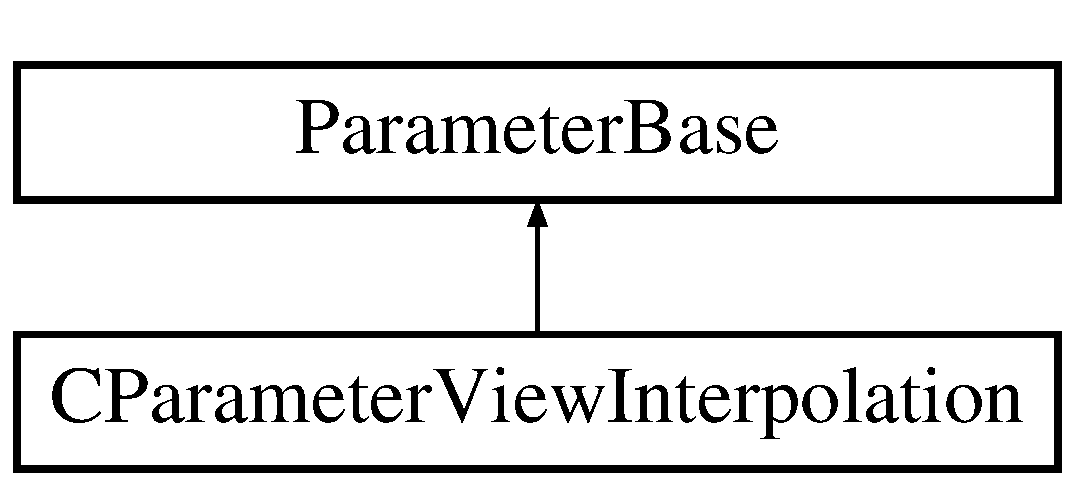
\includegraphics[height=2.000000cm]{class_parameter_base}
\end{center}
\end{figure}
\subsection*{Public Member Functions}
\begin{DoxyCompactItemize}
\item 
\mbox{\Hypertarget{class_parameter_base_a1f149811385414fcf390892910c2d2dd}\label{class_parameter_base_a1f149811385414fcf390892910c2d2dd}} 
virtual Int {\bfseries Init} (Int argc, Char $\ast$$\ast$argv)=0
\item 
\mbox{\Hypertarget{class_parameter_base_a2f9e483f5231ed904f79676c77643a03}\label{class_parameter_base_a2f9e483f5231ed904f79676c77643a03}} 
Int {\bfseries x\+Read\+Line} (F\+I\+LE $\ast$h\+File, std\+::string $\ast$pac\+Tag)
\item 
\mbox{\Hypertarget{class_parameter_base_a6167edf985cccca900b333ace61864e0}\label{class_parameter_base_a6167edf985cccca900b333ace61864e0}} 
Int {\bfseries x\+Read\+From\+File} (std\+::string \&rc\+Filename)
\item 
\mbox{\Hypertarget{class_parameter_base_a3dbbdbf3f40a32470da3b8bfaeb9850b}\label{class_parameter_base_a3dbbdbf3f40a32470da3b8bfaeb9850b}} 
Int {\bfseries x\+Read\+From\+Command\+Line} (Int argc, Char $\ast$$\ast$argv)
\item 
\mbox{\Hypertarget{class_parameter_base_ae0ea9892550a61efaef5ec2e621cc1ac}\label{class_parameter_base_ae0ea9892550a61efaef5ec2e621cc1ac}} 
Int {\bfseries x\+Read\+Command\+Line} (char $\ast$buf, std\+::string $\ast$pac\+Tag)
\item 
\mbox{\Hypertarget{class_parameter_base_a079ee1facad1ead2a6dd14dd25f4b3ae}\label{class_parameter_base_a079ee1facad1ead2a6dd14dd25f4b3ae}} 
Void {\bfseries x\+Print\+Param} ()
\end{DoxyCompactItemize}
\subsection*{Protected Member Functions}
\begin{DoxyCompactItemize}
\item 
\mbox{\Hypertarget{class_parameter_base_adca42e0c992599ac323742a43611c8e3}\label{class_parameter_base_adca42e0c992599ac323742a43611c8e3}} 
virtual U\+Int {\bfseries setup} ()=0
\item 
\mbox{\Hypertarget{class_parameter_base_aae04532a3d349b0d3c8b3cbc8445ad98}\label{class_parameter_base_aae04532a3d349b0d3c8b3cbc8445ad98}} 
Void {\bfseries release} ()
\end{DoxyCompactItemize}
\subsection*{Protected Attributes}
\begin{DoxyCompactItemize}
\item 
\mbox{\Hypertarget{class_parameter_base_a996eee05301784a58fa6bec9d493d0d0}\label{class_parameter_base_a996eee05301784a58fa6bec9d493d0d0}} 
\hyperlink{class_config_line_base}{Config\+Line\+Base} $\ast$ {\bfseries m\+\_\+p\+Cfg\+Lines} \mbox{[}M\+A\+X\+\_\+\+C\+O\+N\+F\+I\+G\+\_\+\+P\+A\+R\+A\+MS\mbox{]}
\end{DoxyCompactItemize}


\subsection{Detailed Description}
\hyperlink{class_parameter_base}{Parameter\+Base}. 

The documentation for this class was generated from the following files\+:\begin{DoxyCompactItemize}
\item 
I\+:/\+V\+S\+R\+S4/vsrs/\+Common\+Lib\+Static/include/Parameter\+Base.\+h\item 
I\+:/\+V\+S\+R\+S4/vsrs/\+Common\+Lib\+Static/src/Parameter\+Base.\+cpp\end{DoxyCompactItemize}

%--- End generated contents ---

% Index
\backmatter
\newpage
\phantomsection
\clearemptydoublepage
\addcontentsline{toc}{chapter}{Index}
\printindex

\end{document}
